\documentclass[]{book}
\usepackage{lmodern}
\usepackage{amssymb,amsmath}
\usepackage{ifxetex,ifluatex}
\usepackage{fixltx2e} % provides \textsubscript
\ifnum 0\ifxetex 1\fi\ifluatex 1\fi=0 % if pdftex
  \usepackage[T1]{fontenc}
  \usepackage[utf8]{inputenc}
\else % if luatex or xelatex
  \ifxetex
    \usepackage{mathspec}
  \else
    \usepackage{fontspec}
  \fi
  \defaultfontfeatures{Ligatures=TeX,Scale=MatchLowercase}
\fi
% use upquote if available, for straight quotes in verbatim environments
\IfFileExists{upquote.sty}{\usepackage{upquote}}{}
% use microtype if available
\IfFileExists{microtype.sty}{%
\usepackage{microtype}
\UseMicrotypeSet[protrusion]{basicmath} % disable protrusion for tt fonts
}{}
\usepackage[margin=1in]{geometry}
\usepackage{hyperref}
\hypersetup{unicode=true,
            pdftitle={¿Cuales son los factores principales y en que proporcion intervienen en el gasto de vivienda de una familia mexicana?},
            pdfauthor={Act. Andrés Antonio Medina Landeros},
            pdfborder={0 0 0},
            breaklinks=true}
\urlstyle{same}  % don't use monospace font for urls
\usepackage{natbib}
\bibliographystyle{apalike}
\usepackage{color}
\usepackage{fancyvrb}
\newcommand{\VerbBar}{|}
\newcommand{\VERB}{\Verb[commandchars=\\\{\}]}
\DefineVerbatimEnvironment{Highlighting}{Verbatim}{commandchars=\\\{\}}
% Add ',fontsize=\small' for more characters per line
\usepackage{framed}
\definecolor{shadecolor}{RGB}{248,248,248}
\newenvironment{Shaded}{\begin{snugshade}}{\end{snugshade}}
\newcommand{\KeywordTok}[1]{\textcolor[rgb]{0.13,0.29,0.53}{\textbf{#1}}}
\newcommand{\DataTypeTok}[1]{\textcolor[rgb]{0.13,0.29,0.53}{#1}}
\newcommand{\DecValTok}[1]{\textcolor[rgb]{0.00,0.00,0.81}{#1}}
\newcommand{\BaseNTok}[1]{\textcolor[rgb]{0.00,0.00,0.81}{#1}}
\newcommand{\FloatTok}[1]{\textcolor[rgb]{0.00,0.00,0.81}{#1}}
\newcommand{\ConstantTok}[1]{\textcolor[rgb]{0.00,0.00,0.00}{#1}}
\newcommand{\CharTok}[1]{\textcolor[rgb]{0.31,0.60,0.02}{#1}}
\newcommand{\SpecialCharTok}[1]{\textcolor[rgb]{0.00,0.00,0.00}{#1}}
\newcommand{\StringTok}[1]{\textcolor[rgb]{0.31,0.60,0.02}{#1}}
\newcommand{\VerbatimStringTok}[1]{\textcolor[rgb]{0.31,0.60,0.02}{#1}}
\newcommand{\SpecialStringTok}[1]{\textcolor[rgb]{0.31,0.60,0.02}{#1}}
\newcommand{\ImportTok}[1]{#1}
\newcommand{\CommentTok}[1]{\textcolor[rgb]{0.56,0.35,0.01}{\textit{#1}}}
\newcommand{\DocumentationTok}[1]{\textcolor[rgb]{0.56,0.35,0.01}{\textbf{\textit{#1}}}}
\newcommand{\AnnotationTok}[1]{\textcolor[rgb]{0.56,0.35,0.01}{\textbf{\textit{#1}}}}
\newcommand{\CommentVarTok}[1]{\textcolor[rgb]{0.56,0.35,0.01}{\textbf{\textit{#1}}}}
\newcommand{\OtherTok}[1]{\textcolor[rgb]{0.56,0.35,0.01}{#1}}
\newcommand{\FunctionTok}[1]{\textcolor[rgb]{0.00,0.00,0.00}{#1}}
\newcommand{\VariableTok}[1]{\textcolor[rgb]{0.00,0.00,0.00}{#1}}
\newcommand{\ControlFlowTok}[1]{\textcolor[rgb]{0.13,0.29,0.53}{\textbf{#1}}}
\newcommand{\OperatorTok}[1]{\textcolor[rgb]{0.81,0.36,0.00}{\textbf{#1}}}
\newcommand{\BuiltInTok}[1]{#1}
\newcommand{\ExtensionTok}[1]{#1}
\newcommand{\PreprocessorTok}[1]{\textcolor[rgb]{0.56,0.35,0.01}{\textit{#1}}}
\newcommand{\AttributeTok}[1]{\textcolor[rgb]{0.77,0.63,0.00}{#1}}
\newcommand{\RegionMarkerTok}[1]{#1}
\newcommand{\InformationTok}[1]{\textcolor[rgb]{0.56,0.35,0.01}{\textbf{\textit{#1}}}}
\newcommand{\WarningTok}[1]{\textcolor[rgb]{0.56,0.35,0.01}{\textbf{\textit{#1}}}}
\newcommand{\AlertTok}[1]{\textcolor[rgb]{0.94,0.16,0.16}{#1}}
\newcommand{\ErrorTok}[1]{\textcolor[rgb]{0.64,0.00,0.00}{\textbf{#1}}}
\newcommand{\NormalTok}[1]{#1}
\usepackage{longtable,booktabs}
\usepackage{graphicx,grffile}
\makeatletter
\def\maxwidth{\ifdim\Gin@nat@width>\linewidth\linewidth\else\Gin@nat@width\fi}
\def\maxheight{\ifdim\Gin@nat@height>\textheight\textheight\else\Gin@nat@height\fi}
\makeatother
% Scale images if necessary, so that they will not overflow the page
% margins by default, and it is still possible to overwrite the defaults
% using explicit options in \includegraphics[width, height, ...]{}
\setkeys{Gin}{width=\maxwidth,height=\maxheight,keepaspectratio}
\IfFileExists{parskip.sty}{%
\usepackage{parskip}
}{% else
\setlength{\parindent}{0pt}
\setlength{\parskip}{6pt plus 2pt minus 1pt}
}
\setlength{\emergencystretch}{3em}  % prevent overfull lines
\providecommand{\tightlist}{%
  \setlength{\itemsep}{0pt}\setlength{\parskip}{0pt}}
\setcounter{secnumdepth}{5}
% Redefines (sub)paragraphs to behave more like sections
\ifx\paragraph\undefined\else
\let\oldparagraph\paragraph
\renewcommand{\paragraph}[1]{\oldparagraph{#1}\mbox{}}
\fi
\ifx\subparagraph\undefined\else
\let\oldsubparagraph\subparagraph
\renewcommand{\subparagraph}[1]{\oldsubparagraph{#1}\mbox{}}
\fi

%%% Use protect on footnotes to avoid problems with footnotes in titles
\let\rmarkdownfootnote\footnote%
\def\footnote{\protect\rmarkdownfootnote}

%%% Change title format to be more compact
\usepackage{titling}

% Create subtitle command for use in maketitle
\newcommand{\subtitle}[1]{
  \posttitle{
    \begin{center}\large#1\end{center}
    }
}

\setlength{\droptitle}{-2em}

  \title{¿Cuales son los factores principales y en que proporcion intervienen en
el gasto de vivienda de una familia mexicana?}
    \pretitle{\vspace{\droptitle}\centering\huge}
  \posttitle{\par}
    \author{Act. Andrés Antonio Medina Landeros}
    \preauthor{\centering\large\emph}
  \postauthor{\par}
      \predate{\centering\large\emph}
  \postdate{\par}
    \date{2018-07-24}

\usepackage{booktabs}
\usepackage{amsthm}
\makeatletter
\def\thm@space@setup{%
  \thm@preskip=8pt plus 2pt minus 4pt
  \thm@postskip=\thm@preskip
}
\makeatother

\begin{document}
\maketitle

{
\setcounter{tocdepth}{1}
\tableofcontents
}
\begin{Shaded}
\begin{Highlighting}[]
\KeywordTok{install.packages}\NormalTok{(}\StringTok{"bookdown"}\NormalTok{)}
\CommentTok{# or the development version}
\CommentTok{# devtools::install_github("rstudio/bookdown")}
\end{Highlighting}
\end{Shaded}

\chapter{Abstracto}\label{abstracto}

Esta investigacion tiene como objetivo conocer y cuantificar el impacto
que tienen en el gasto en vivienda los factores mas relevantes del
entorno socio economico y demografico de las familias mexicanas. Como
resultado de este estudio encontre patrones linealmente positivos pero
marginalmente decrecientes del gasto mensual y la edad del jefe de
familia con respecto del gasto en vivienda. Encontre que el sexo del
jefe de familia tambien afecta los patrones de consumo en vivienda, el
estudio demuestra que los hombres gastan menos dinero en este concepto
que las mujeres. Por ultimo, descubri que existe una relacion lineal
positiva entre el estrato socio economico al que pertenece la unidad de
analisis y su patron de consumo de vivienda, este efecto positivo puede
ser descrito como que, entre mas alto el estrato al que pertenece, mas
dinero destina esa familia a la vivienda. La metodoligia que implemente
en este estudio es la construccion de un modelo de regresion lineal
multiple generalizado.

\chapter{Introduccion}\label{introduccion}

La teoria economica nos ha presentado un marco teorico en el cual se
incluye la forma en la que el mercado de vivienda contribuye a propulsar
el dinamismo economico. algunas de las formas mas importantes en las que
la vivienda logra impactar a los mexicanos son, por ejemplo la derrama
economica que genera en otros sectores de la economia, y en la medida en
que permite el desarrollo de otros aspectos del ser humano que le
permiten mejorar sus condiciones socio economicas, sin embargo la
industria inmobiliaria, por diversos factores ha sido descrita como
inflexible, inamovible, firme, e inapelable por lo que en muchos
mercados, el sector no ha podido generar soluciones de valor para su
consumidor final. Ha llegado el momento de implantarle un nuevo
dinamismo a la industria mediante la implementacion de la inteligencia
de negocios.

Muchos de los procesos que URBI utiliza para prospectar y cuantificar
sus mercados meta y el valor de estos son obsoletos, apoyados en
hipotesis que carecen de sustento frente a una realidad mexicana
constanemente cambiante, estas hipotesis deben ser puestas a prueba y
contrastadas con datos para encontrar nuevas ideas y soluciones que
entreguen valor a nuestrso clientes.

El enfoque que presento en este trabajo esta centrado en la familia
mexicana como unidad de analisis, quiero conocer y cuantificar los
patrones de consumo en este bien, esto, con el proposito de que URBI,
como empresa tenga un panorama general, apoyado en datos sobre quienes
son las personas que destinan sus recursos en nuestras soluciones
integrales de vivienda, de tal forma que URBI pueda adaptar su gama de
productos y servicios a la realidad de nuestros clientes.

Es claro que la aproximacion que utilice en la presente investigacion no
es del tipo exhaustivo, sino mas bien quiero presentarles mis hallazgos
para que en conjunto tomemos conciencia del importante poder descriptivo
y predictivo que nos provee esta clase de modelacion estadistica con
miras a que en un futuro, mejoremos nuestros procesos de interacci?n con
los clientes, procesos en los cuales recabemos, almacenemos y procesemos
de forma valiosa la informacion.

\chapter{Datos}\label{datos}

los datos utilizados en este proyecto son los proporcionados por la
Encuesta Nacional Ingresos y Gastos de los hogares en su edicion 2016
(ENIGH 2016). El objetivo de esta encuesta es el de proporcionar un
panorama estadistico del comportamiento de los ingresos y gastos de los
hogares en cuanto a su monto, procedencia y distribucion, adicionalmente
la encuesta ofrece caracteristicas ocupacionales y socio demograficas de
la infraestructura de la vivienda y el equipamiento del hogar. El
periodo de levantamiento de la encuesta fue del 21 de Agosto del 2016 al
28 de noviembre del 2016. La cobertura geografica de la encuesta es a
nivel nacional.

Para conformar la base de datos de la investigacion utilice el archivo
concentradohogar.csv que se encuentra disponible en la pestana de
microdatos en el sitio web de la
\href{http://www.beta.inegi.org.mx/proyectos/enchogares/regulares/enigh/nc/2016/}{ENIGH}

\section{Descripcion de las
variables}\label{descripcion-de-las-variables}

A continuacion, presento una tabla de las variables que conforman la
base de datos utilizada en este analisis, el numero significa la columna
en la que se encuentran en el archivo, su nombre, su etiqueta, su
categoria (si es numerica o categorica) y en caso de ser categorica el
numero de niveles que la conforman. El archivo se compone de 70,311
unidades observacionales, de las cuales seleccione 1000 mediante un
muestreo aleatorio y omiti de la base aquellos cuyo gasto en vivienda
reportado es del orden de centavos, ya que estos datos no tienen ningun
sentido economico ni financiero y claramente son errores de
captura.Gracias al procedimiento anteriormente mencionado me quedo con
969 unidades para realizar el analisis.

\begin{table}

\caption{\label{tab:unnamed-chunk-7}Tabla de variables a utilizar.}
\centering
\begin{tabular}[t]{r|l|l|l}
\hline
Numero & variable & etiqueta & unidades\\
\hline
6 & estsocio & estrato socio economico & categorica, con niveles de 1 a 4\\
\hline
11 & sexojefe & sexo del jefe de familia & categorica con niveles 0 o 1\\
\hline
12 & educajefe & educacion formal del jefe de familia & categorica con niveles 1 a 11\\
\hline
13 & totinteg & numero de integrantes del hogar & numerica\\
\hline
14 & ingcor & ingreso corriente trimestral de la unidad de observacion & numerica\\
\hline
58 & gastomon & gasto corriente trimestral de la unidad de observacion & numerica\\
\hline
80 & vivienda & gasto en vivienda trimestral, se incluye renta o pago de hipoteca, gasto en servicios de reconstruccion y en agua & numerica\\
\hline
\end{tabular}
\end{table}

\begin{table}

\caption{\label{tab:unnamed-chunk-8} niveles de la variable categorica sexo del jefe de familia.}
\centering
\begin{tabular}[t]{r|l}
\hline
Valor & Etiqueta\\
\hline
0 & Mujer\\
\hline
1 & Hombre\\
\hline
\end{tabular}
\end{table}

\begin{table}

\caption{\label{tab:unnamed-chunk-8} niveles de la variable categorica estrato socio-economico.}
\centering
\begin{tabular}[t]{r|l}
\hline
Valor & Etiqueta\\
\hline
1 & Bajo\\
\hline
2 & Medio Bajo\\
\hline
3 & Medio Alto\\
\hline
4 & Alto\\
\hline
\end{tabular}
\end{table}

\begin{table}

\caption{\label{tab:unnamed-chunk-8} niveles de la variable categorica educacion formal del jefe de familia.}
\centering
\begin{tabular}[t]{r|l}
\hline
Valor & Etiqueta\\
\hline
1 & sin instruccion\\
\hline
2 & preescolar\\
\hline
3 & primaria incompleta\\
\hline
4 & primaria completa\\
\hline
5 & secundaria incompleta\\
\hline
6 & secundaria completa\\
\hline
7 & preparatoria incompleta\\
\hline
8 & preparatoria completa\\
\hline
9 & profesional incompleta\\
\hline
10 & profesional completa\\
\hline
11 & posgrado\\
\hline
\end{tabular}
\end{table}

\chapter{Analisis exploratorio de los datos y estadistica
descrpitiva}\label{analisis-exploratorio-de-los-datos-y-estadistica-descrpitiva}

El analisis exploratorio de los datos consiste en descubrir las
relaciones entre las variables propuestas para el modelo, para que asi
se puedan presentar de forma correcta. Tambien es util para conocer la
estructura de los datos y conocer su consistencia. La forma en la que
presento esta seccion es primero, con estadisticas descrptivas de las
variables numericas, entre las cuales se incluyen media, moda,
desviacion estandard, cuartiles, minimo y maximo. A continuacion prosigo
con graficas de estadistica univariada, entre los que se incluyen,
diagramas de caja y brazos, histogramas y graficos de densidad esto con
el proposito de conocer la forma, el sesgo y los parametros de
localizacion de la distribucion de estas variables. Despues exploro
algunas relaciones multivariadas entre distintos parametros categoricos
y numericos, esto con el fin de conocer las caracteristicas de la
poblacion.

\section{Estadistica Descriptiva}\label{estadistica-descriptiva}

\begin{longtable}[]{@{}ll@{}}
\toprule
& datos2 (N = 969)\tabularnewline
\midrule
\endhead
\textbf{Edad del jefe de familia} & ~~\tabularnewline
~~ min & 17\tabularnewline
~~ median (IQR) & 47 (37.00, 61.00)\tabularnewline
~~ mean (sd) & 49.28 ± 16.41\tabularnewline
~~ max & 104\tabularnewline
\textbf{Total de integrantes del hogar} & ~~\tabularnewline
~~ min & 1\tabularnewline
~~ median (IQR) & 3 (2.00, 5.00)\tabularnewline
~~ mean (sd) & 3.65 ± 1.83\tabularnewline
~~ max & 11\tabularnewline
\textbf{Gasto general(log)} & ~~\tabularnewline
~~ min & 6.061783\tabularnewline
~~ median (IQR) & 9.89 (9.42, 10.36)\tabularnewline
~~ mean (sd) & 9.89 ± 0.79\tabularnewline
~~ max & 12.5858\tabularnewline
\textbf{Ingreso(log)} & ~~\tabularnewline
~~ min & 7.280429\tabularnewline
~~ median (IQR) & 10.36 (9.82, 10.88)\tabularnewline
~~ mean (sd) & 10.35 ± 0.80\tabularnewline
~~ max & 13.8962\tabularnewline
\textbf{Gasto en vivienda(log)} & ~~\tabularnewline
~~ min & 3.218876\tabularnewline
~~ median (IQR) & 7.34 (6.69, 7.88)\tabularnewline
~~ mean (sd) & 7.27 ± 1.08\tabularnewline
~~ max & 10.47658\tabularnewline
\bottomrule
\end{longtable}

\section{Analisis Univariado}\label{analisis-univariado}

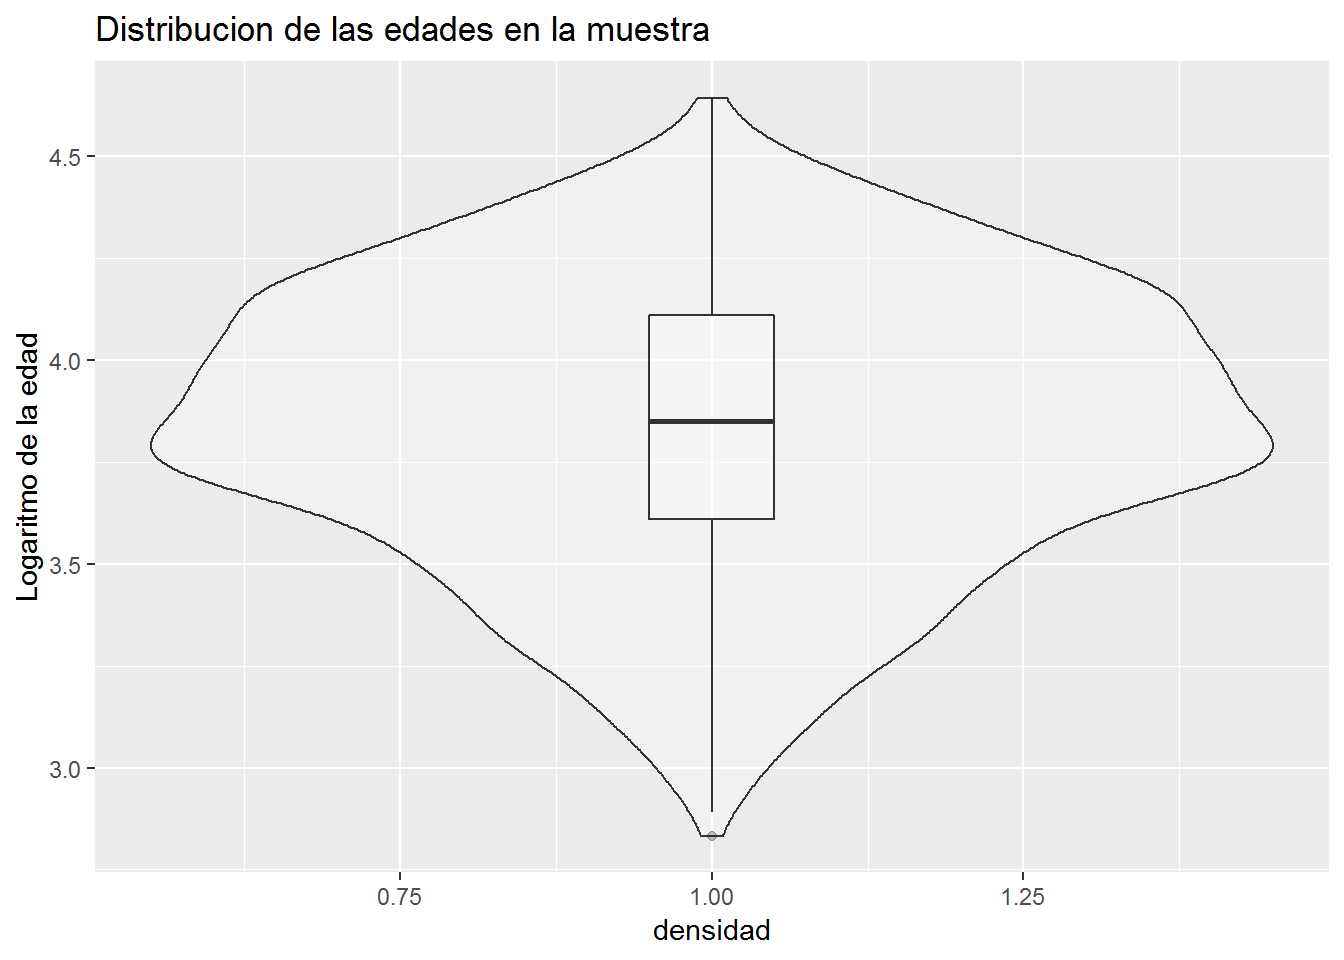
\includegraphics{bookdown-demo_files/figure-latex/unnamed-chunk-10-1.pdf}

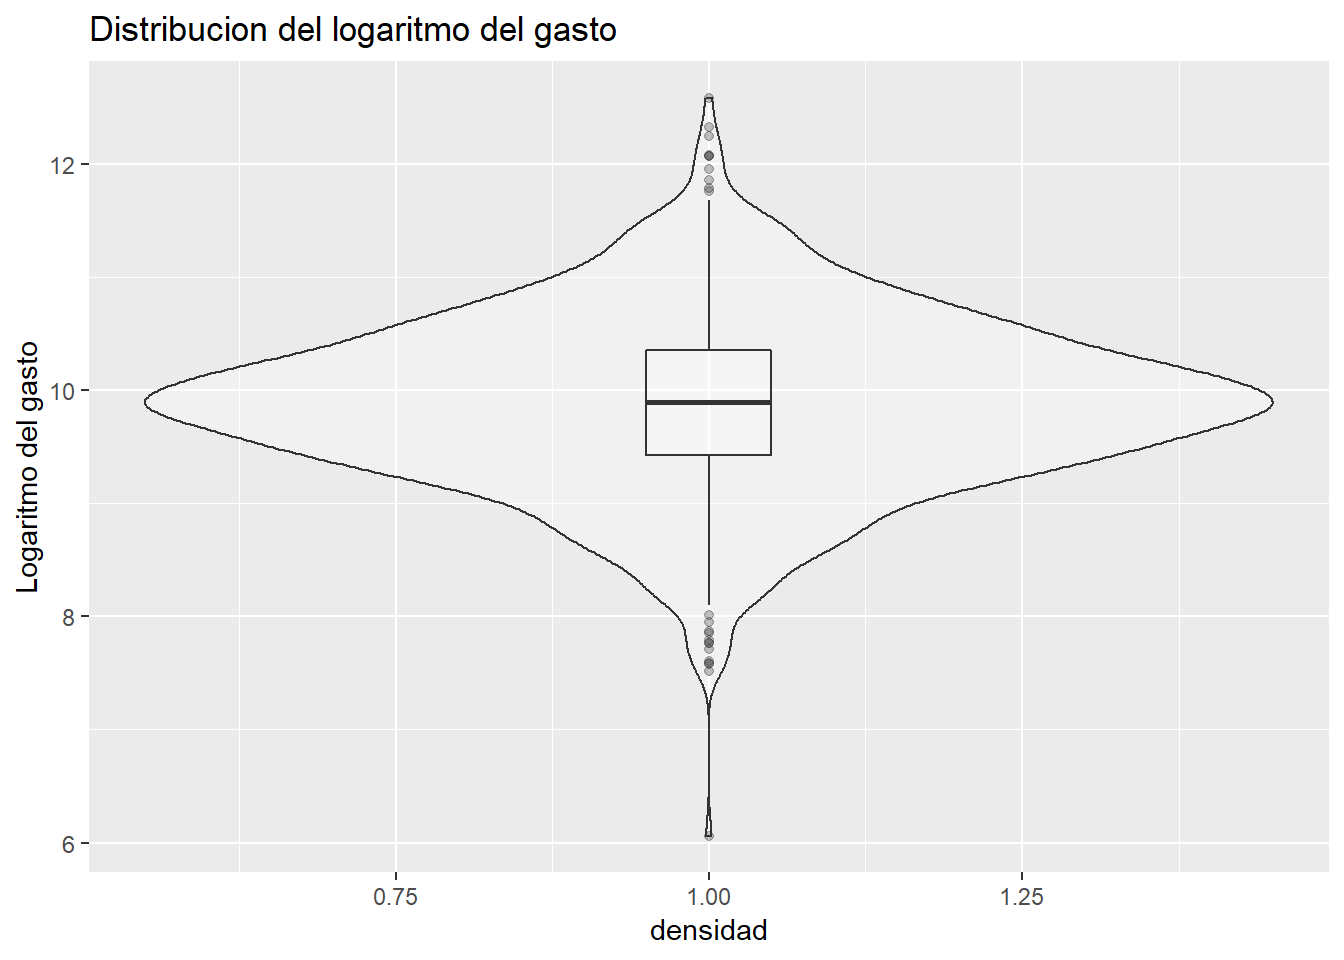
\includegraphics{bookdown-demo_files/figure-latex/unnamed-chunk-11-1.pdf}

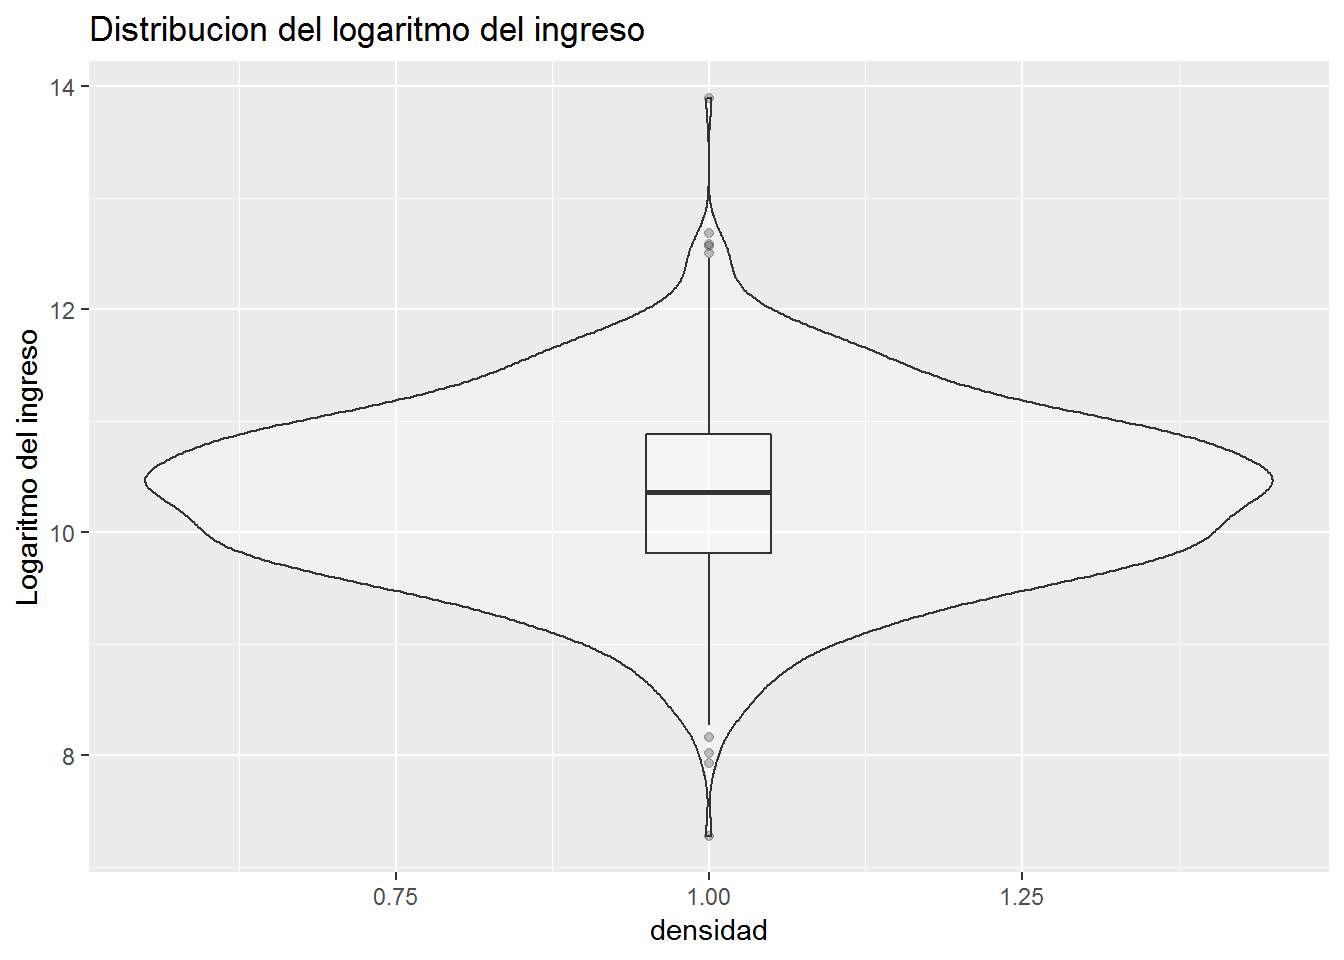
\includegraphics{bookdown-demo_files/figure-latex/unnamed-chunk-12-1.pdf}

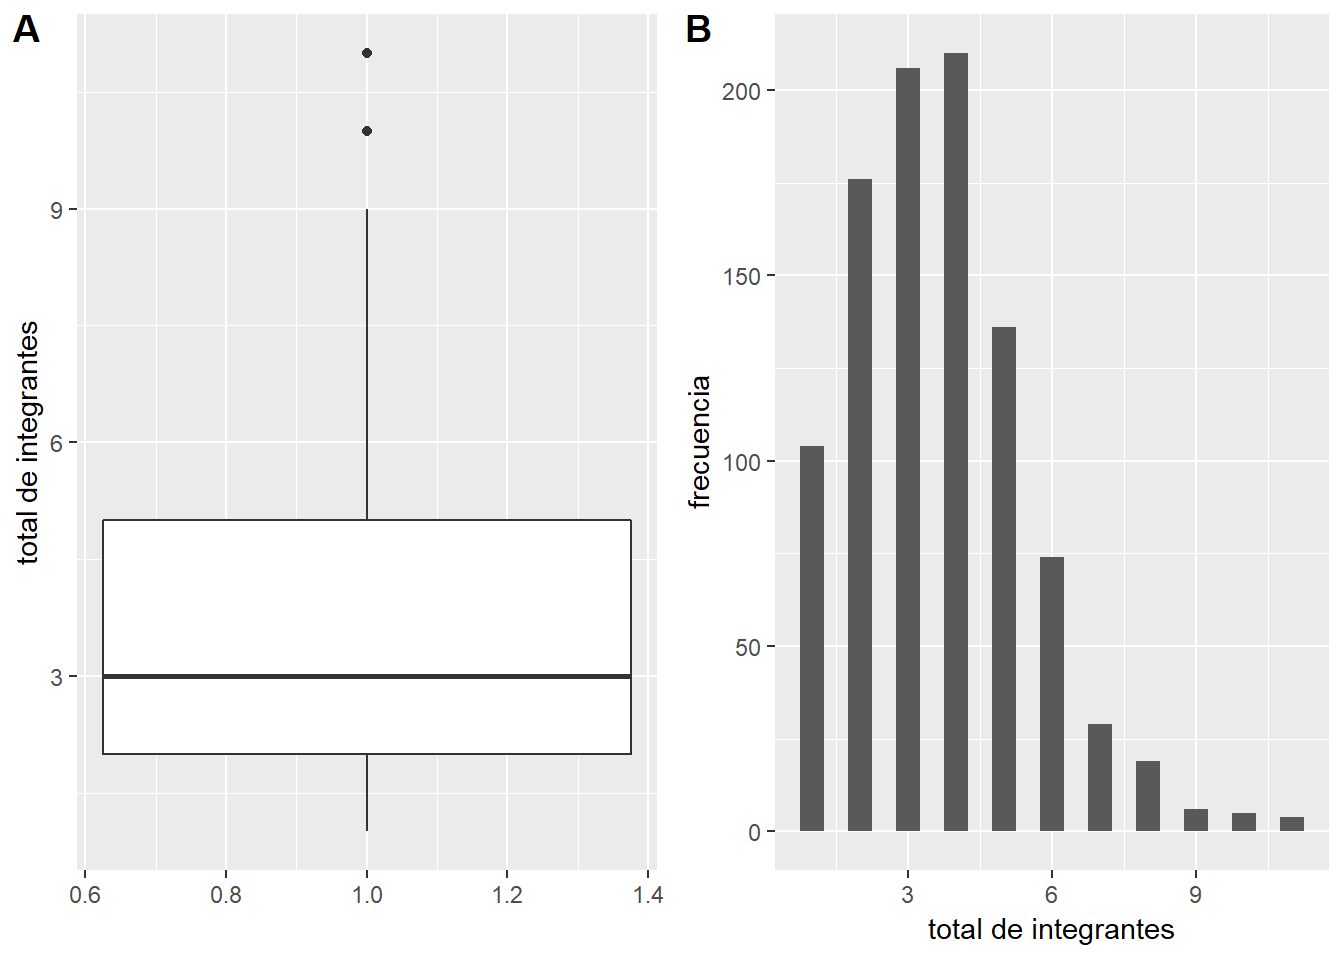
\includegraphics{bookdown-demo_files/figure-latex/unnamed-chunk-13-1.pdf}

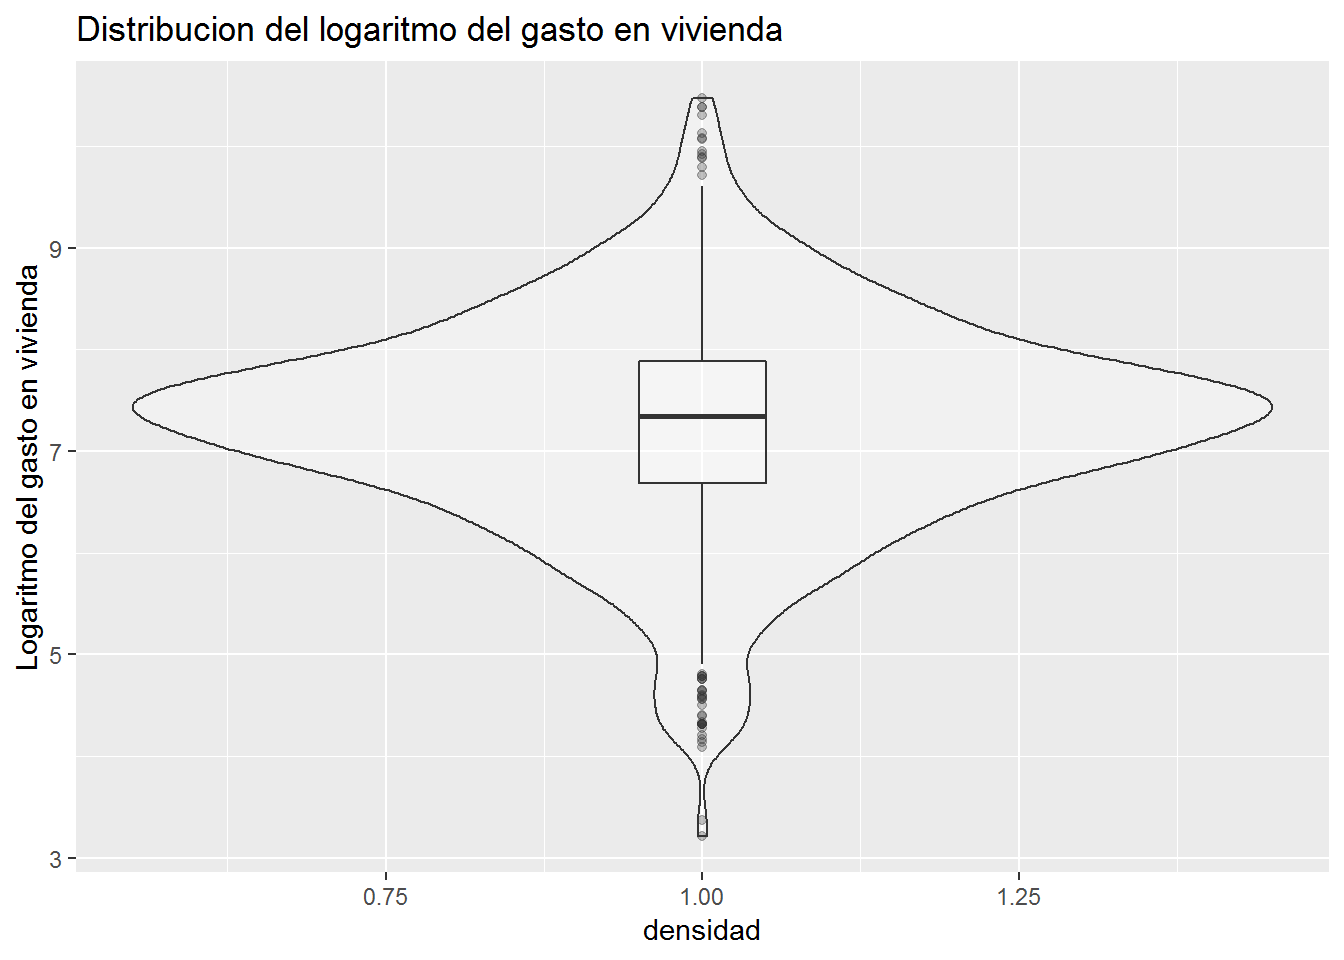
\includegraphics{bookdown-demo_files/figure-latex/unnamed-chunk-14-1.pdf}

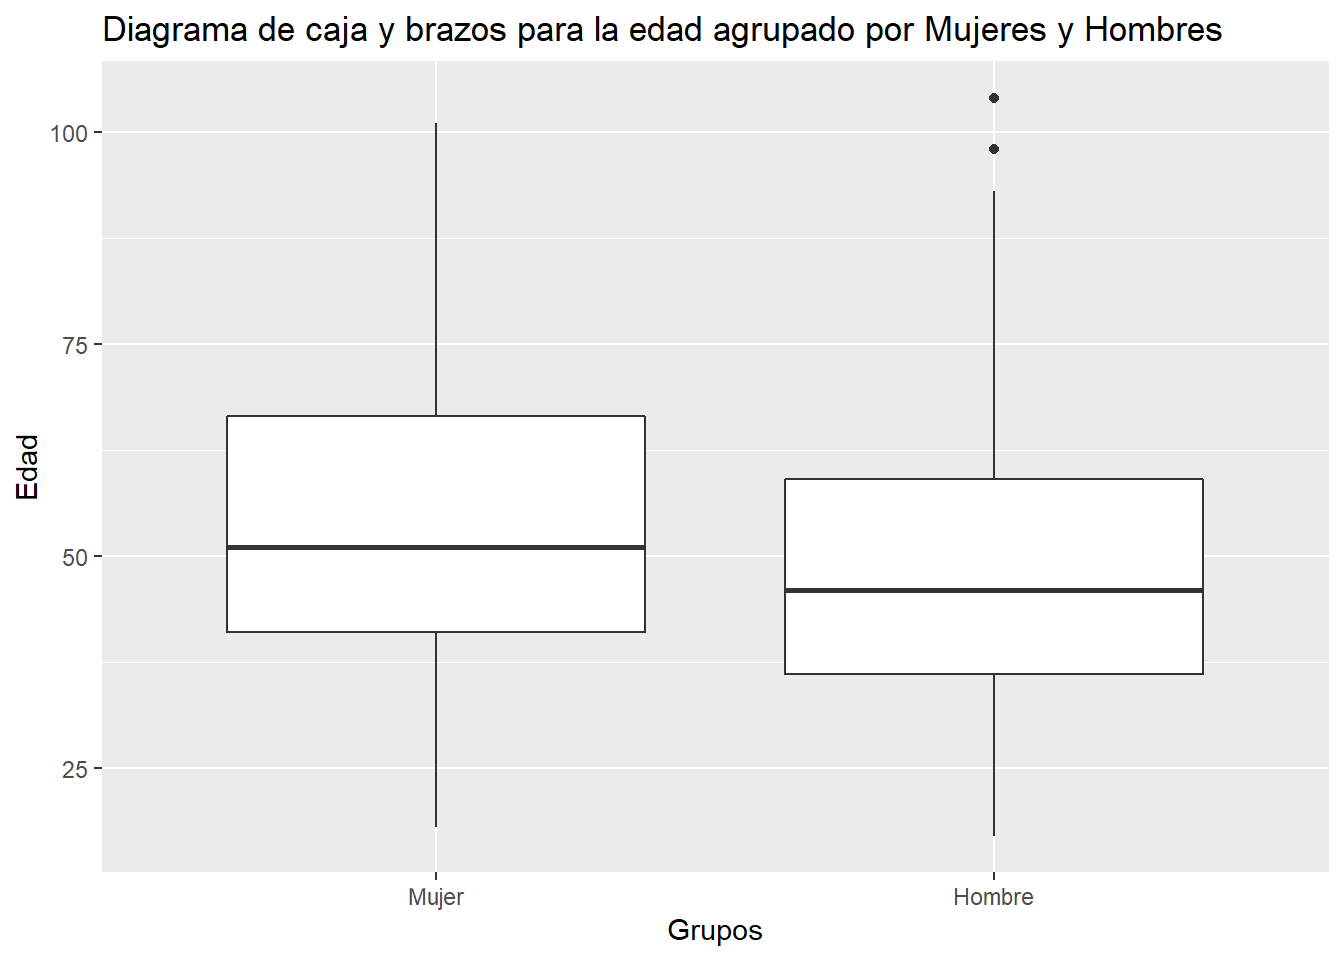
\includegraphics{bookdown-demo_files/figure-latex/unnamed-chunk-15-1.pdf}

\section{Analisis Multivariado}\label{analisis-multivariado}

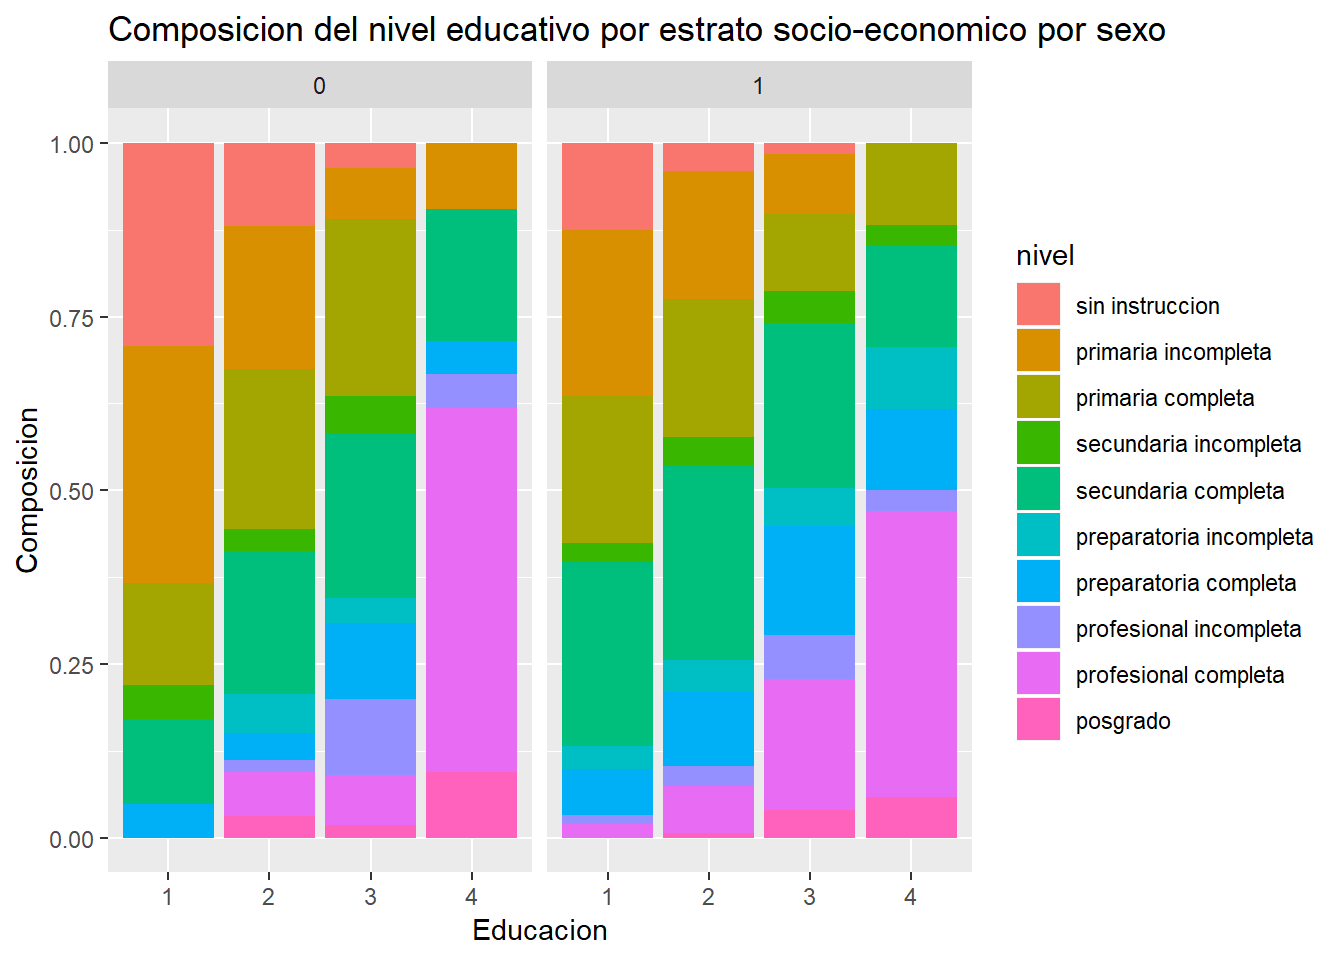
\includegraphics{bookdown-demo_files/figure-latex/unnamed-chunk-17-1.pdf}

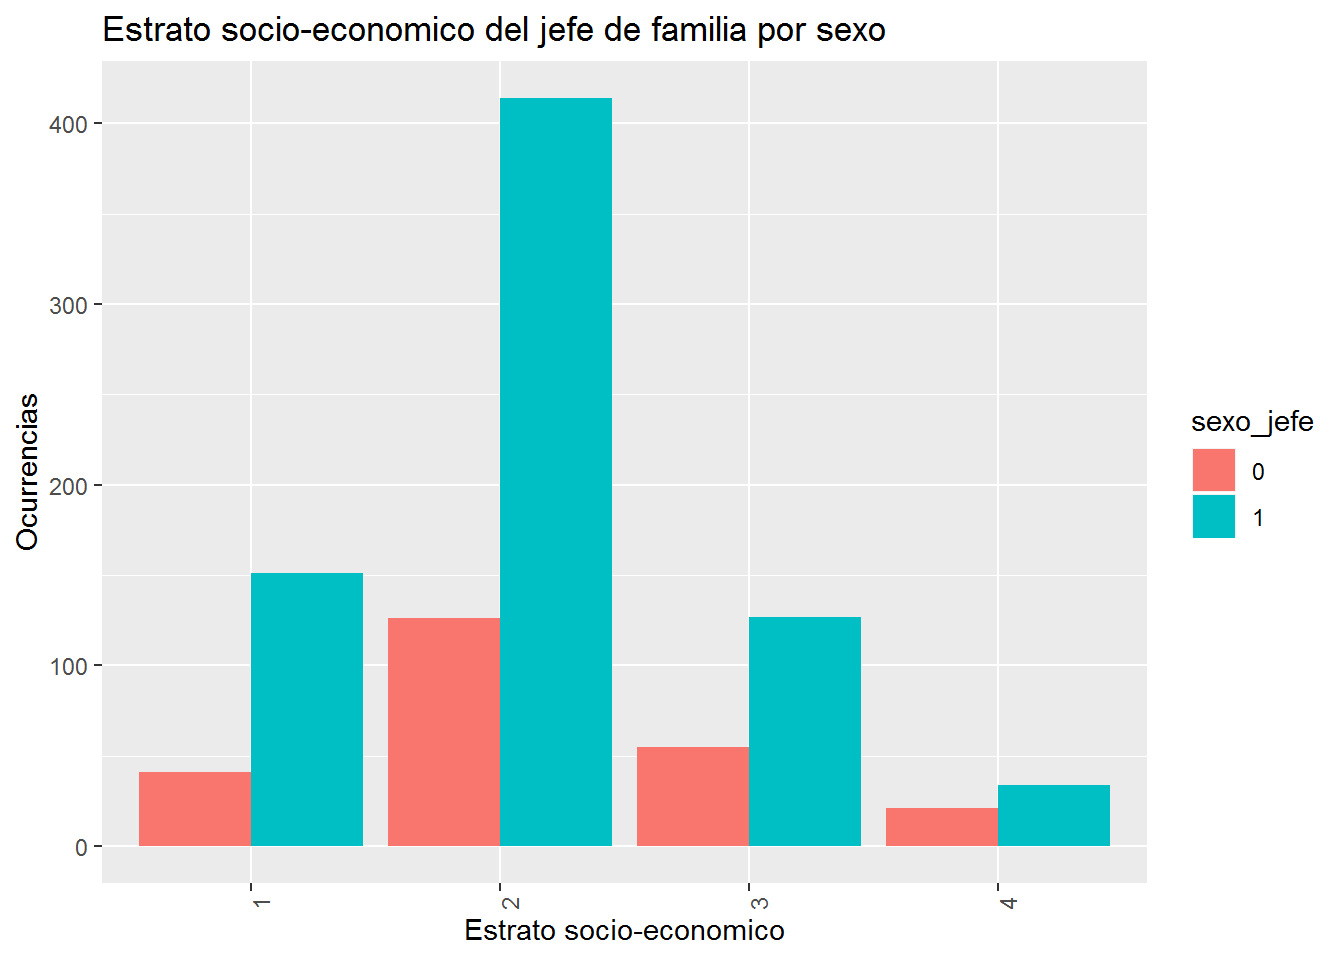
\includegraphics{bookdown-demo_files/figure-latex/unnamed-chunk-18-1.pdf}

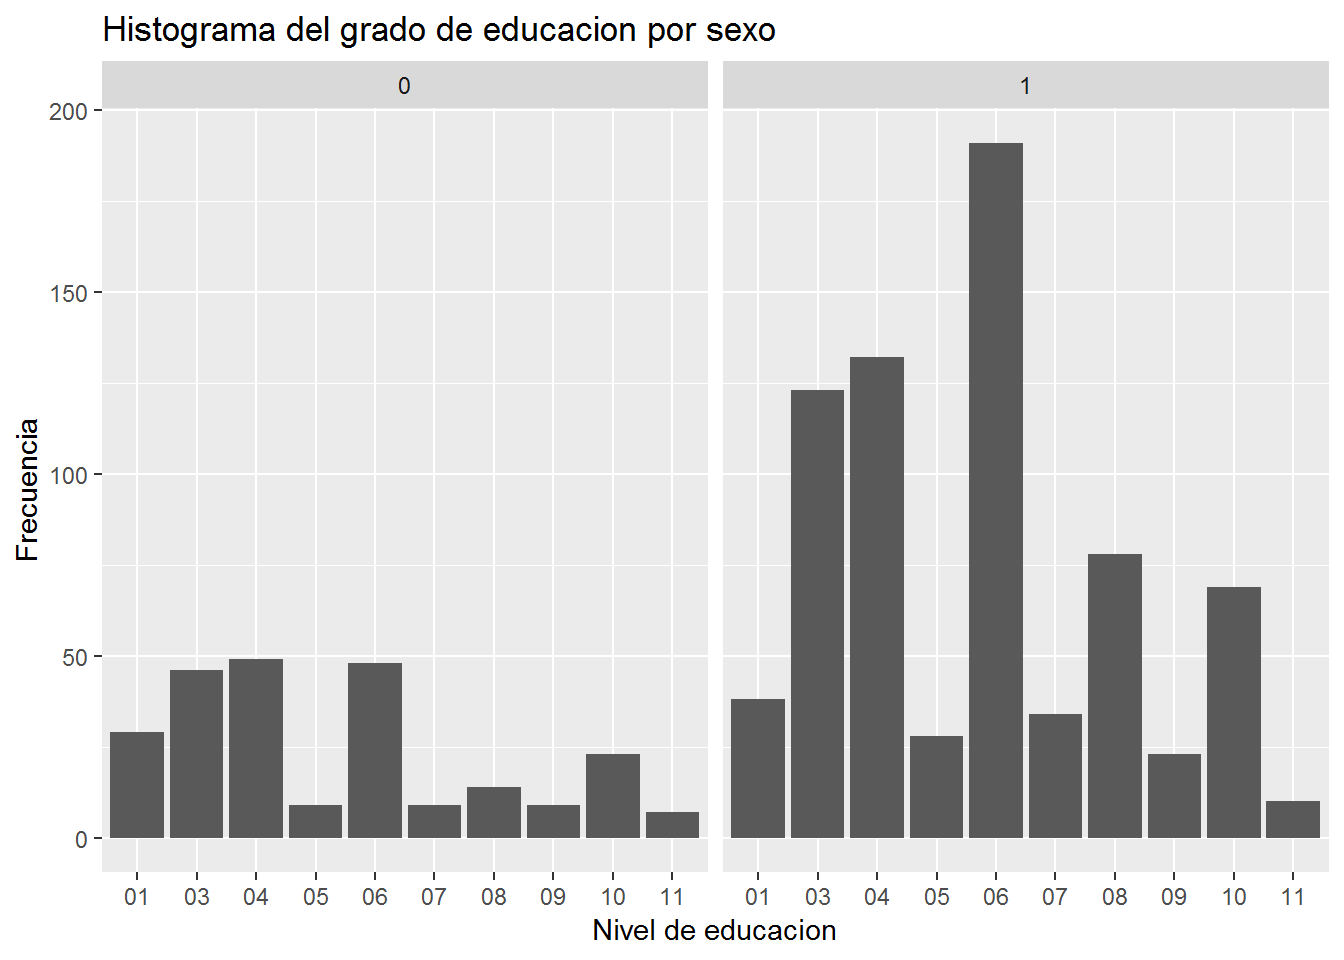
\includegraphics{bookdown-demo_files/figure-latex/unnamed-chunk-19-1.pdf}

\subsection{Relaciones entre regresores y variable
explicada}\label{relaciones-entre-regresores-y-variable-explicada}

\subsubsection{Diagramas de relacion
lineal}\label{diagramas-de-relacion-lineal}

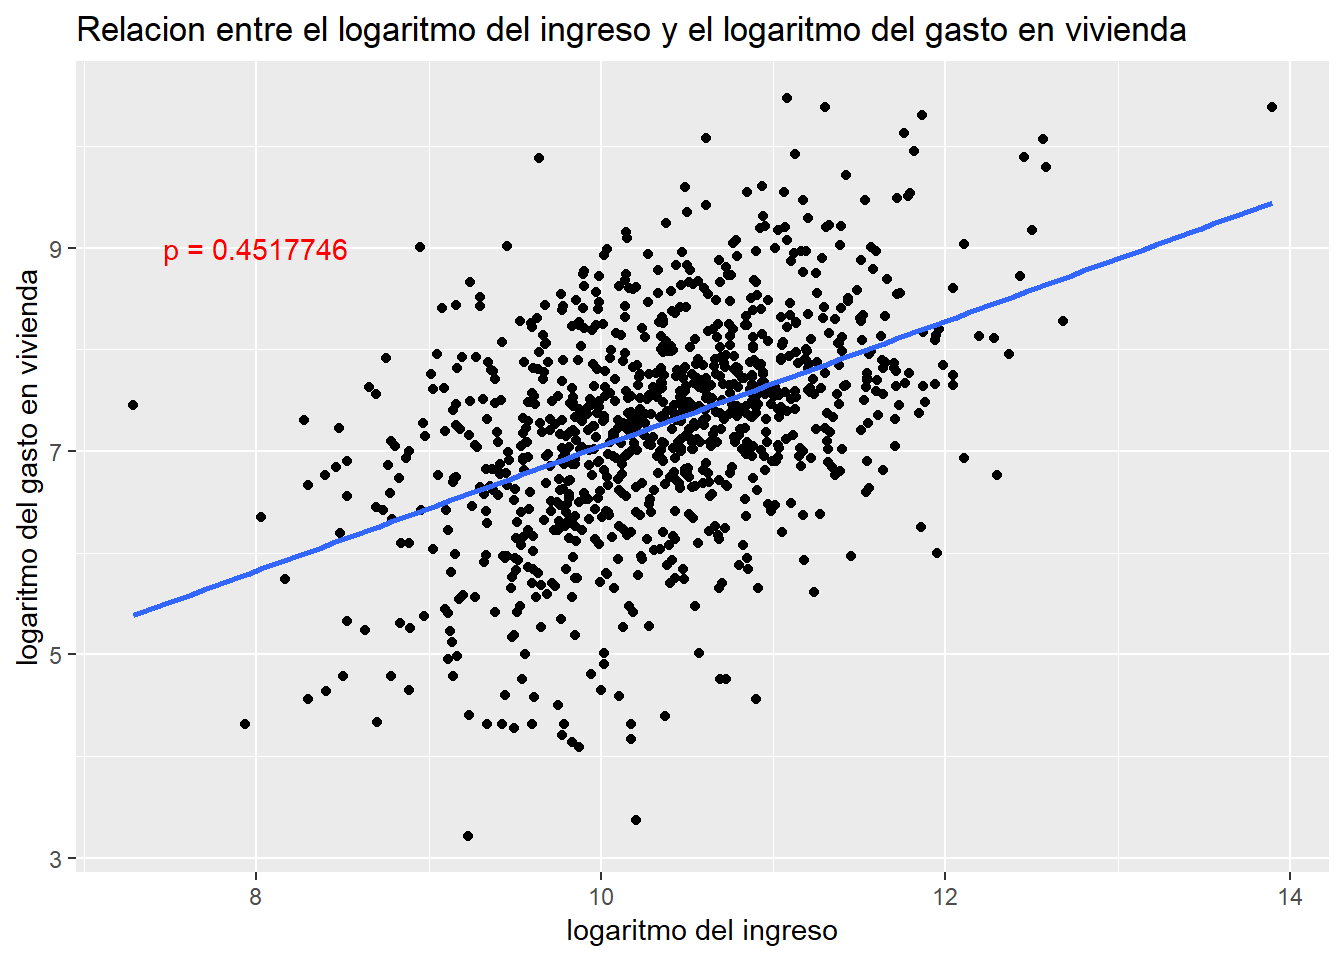
\includegraphics{bookdown-demo_files/figure-latex/unnamed-chunk-21-1.pdf}
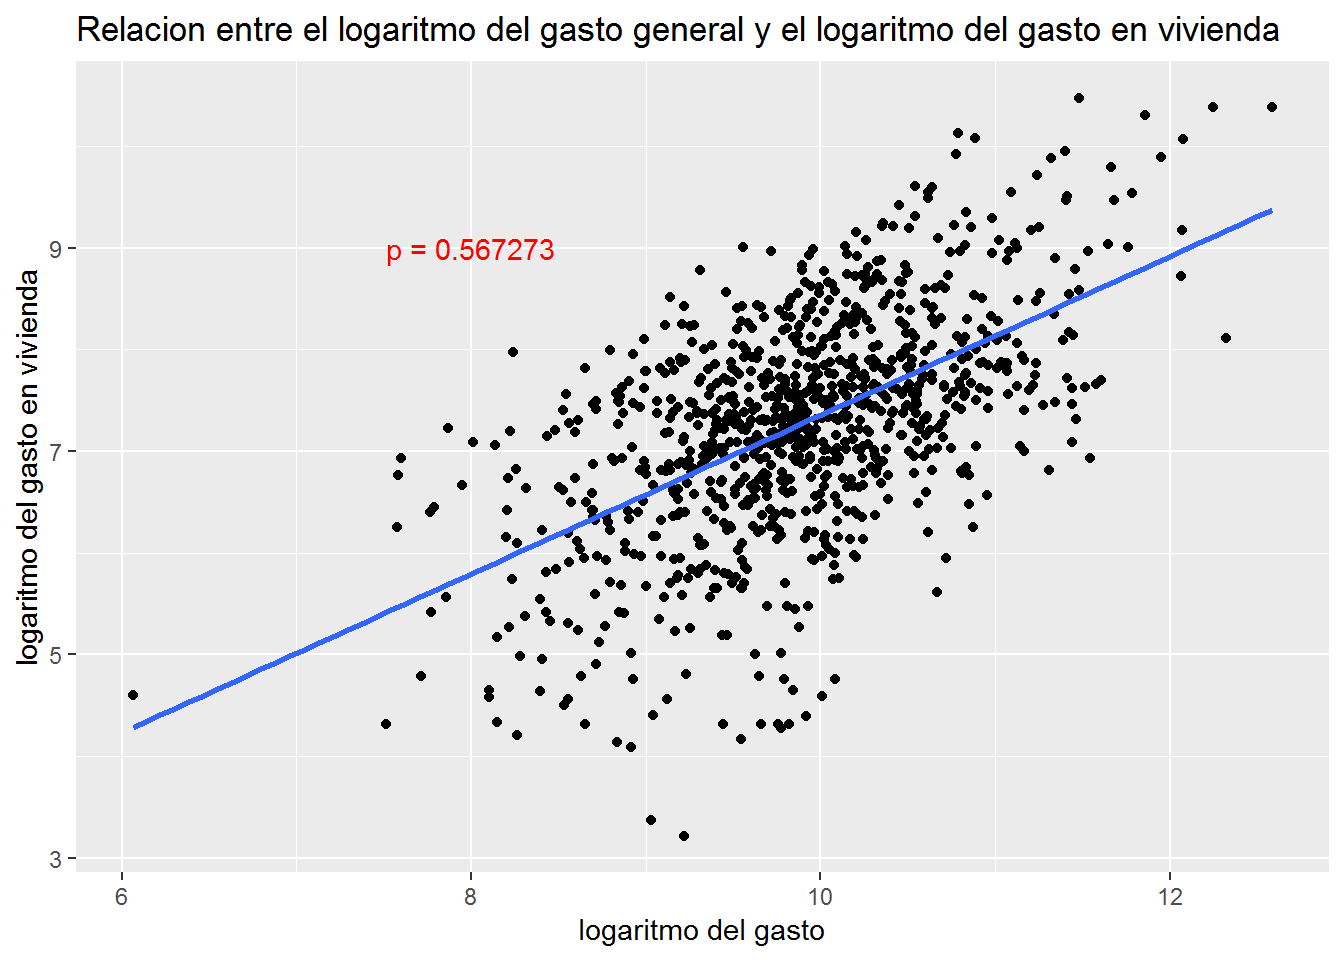
\includegraphics{bookdown-demo_files/figure-latex/unnamed-chunk-21-2.pdf}
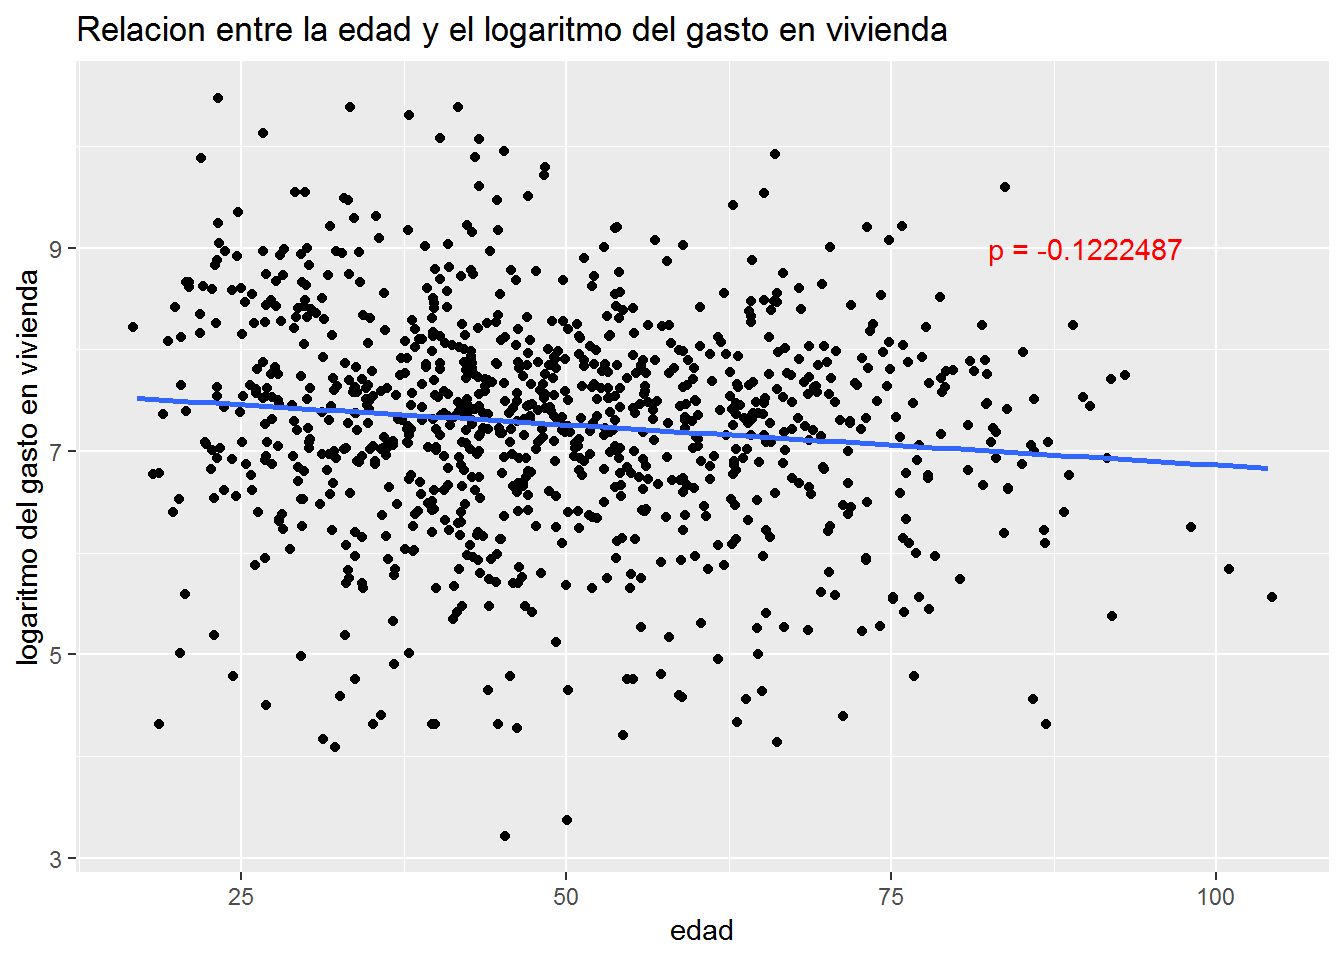
\includegraphics{bookdown-demo_files/figure-latex/unnamed-chunk-21-3.pdf}

\subsubsection{Distribucion del gasto en vivienda agrupado por
sexo}\label{distribucion-del-gasto-en-vivienda-agrupado-por-sexo}

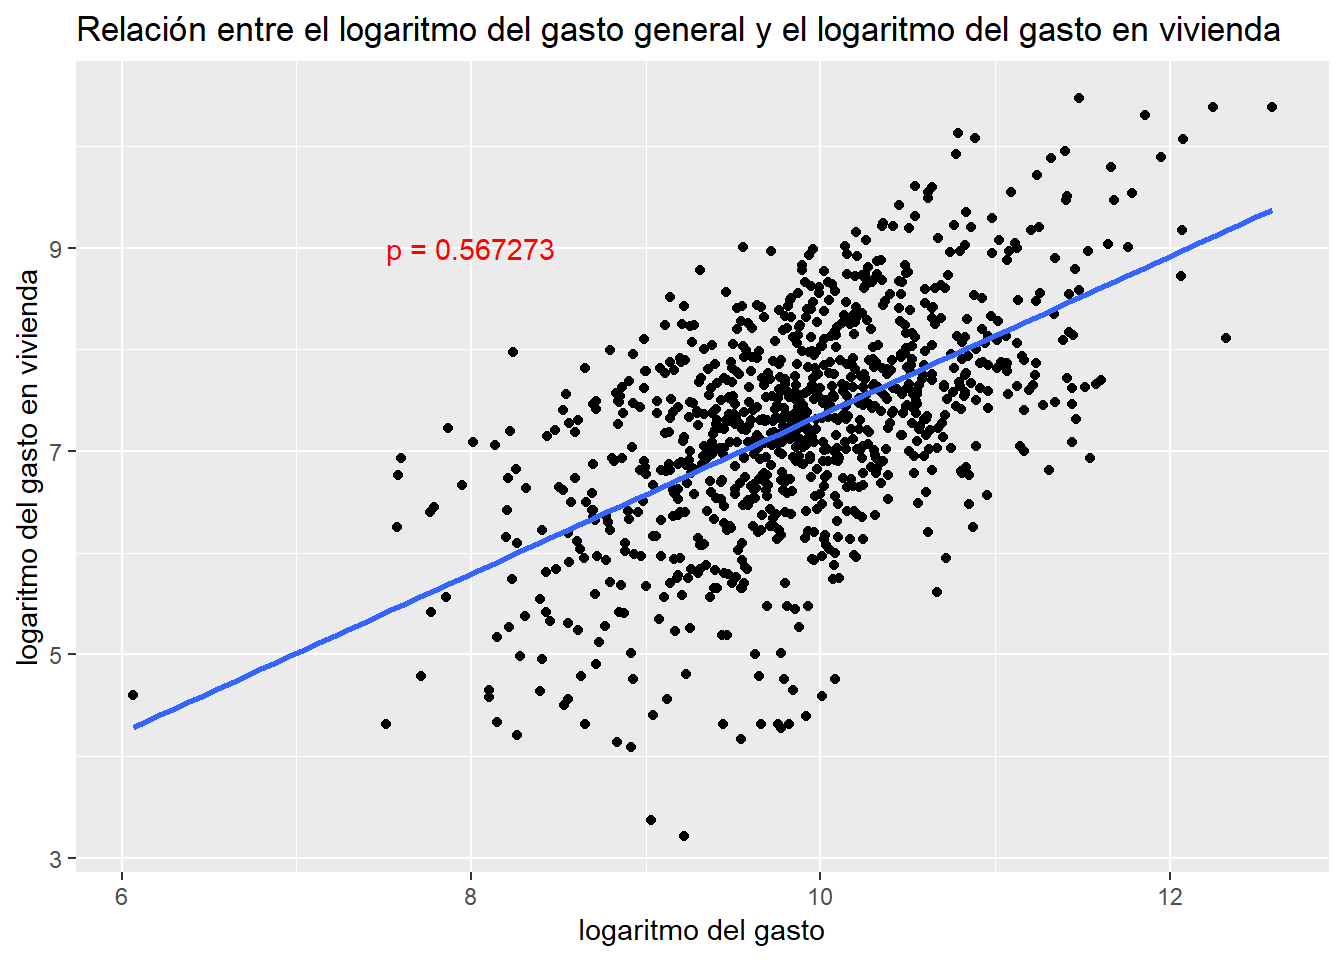
\includegraphics{bookdown-demo_files/figure-latex/unnamed-chunk-22-1.pdf}
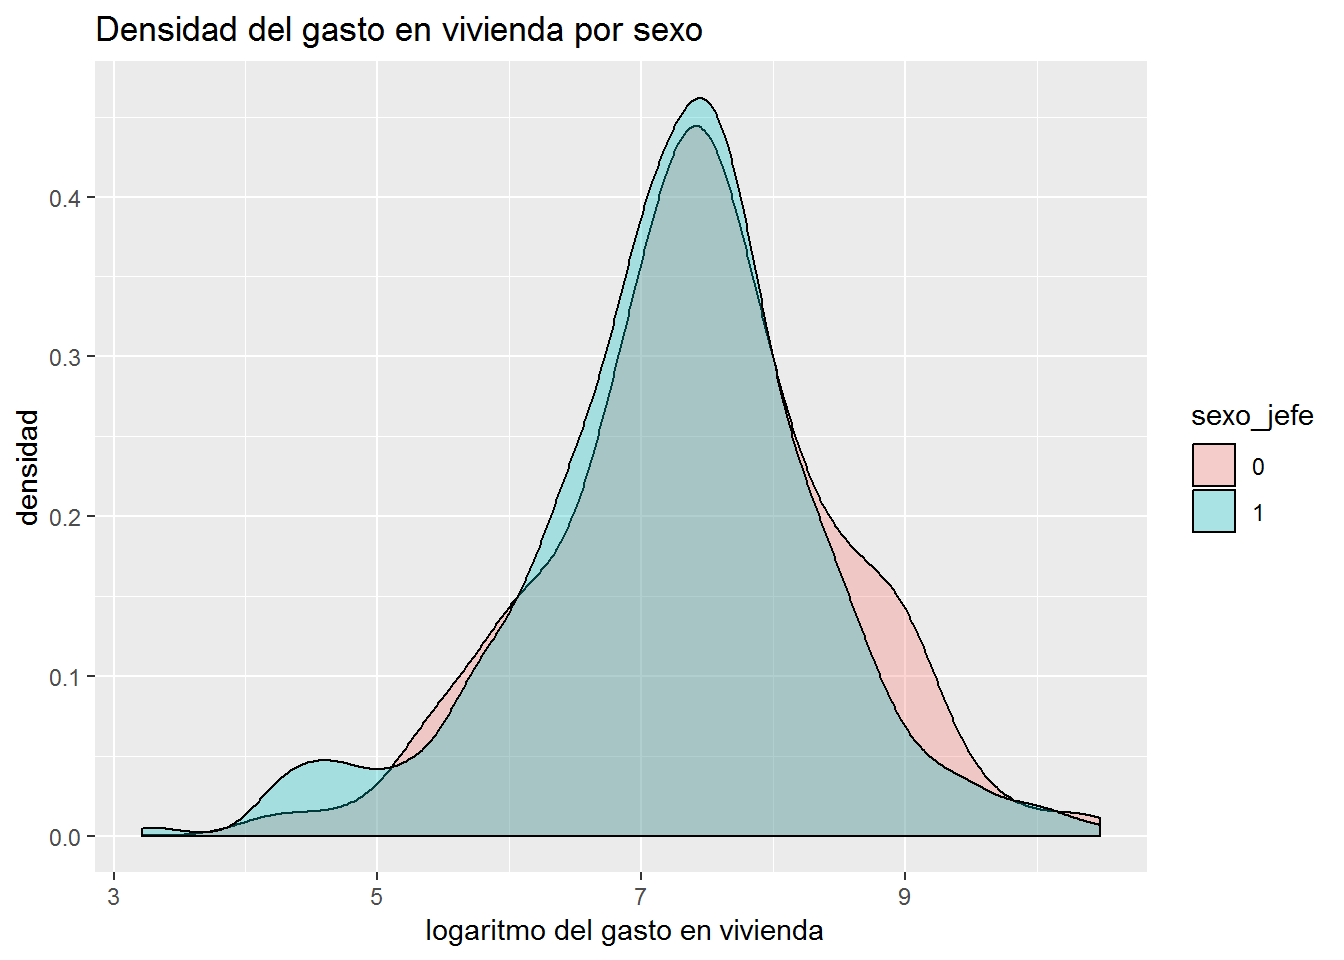
\includegraphics{bookdown-demo_files/figure-latex/unnamed-chunk-22-2.pdf}

\subsubsection{Distribucion del gasto en vivienda agrupado por total de
integrantes del
hogar}\label{distribucion-del-gasto-en-vivienda-agrupado-por-total-de-integrantes-del-hogar}

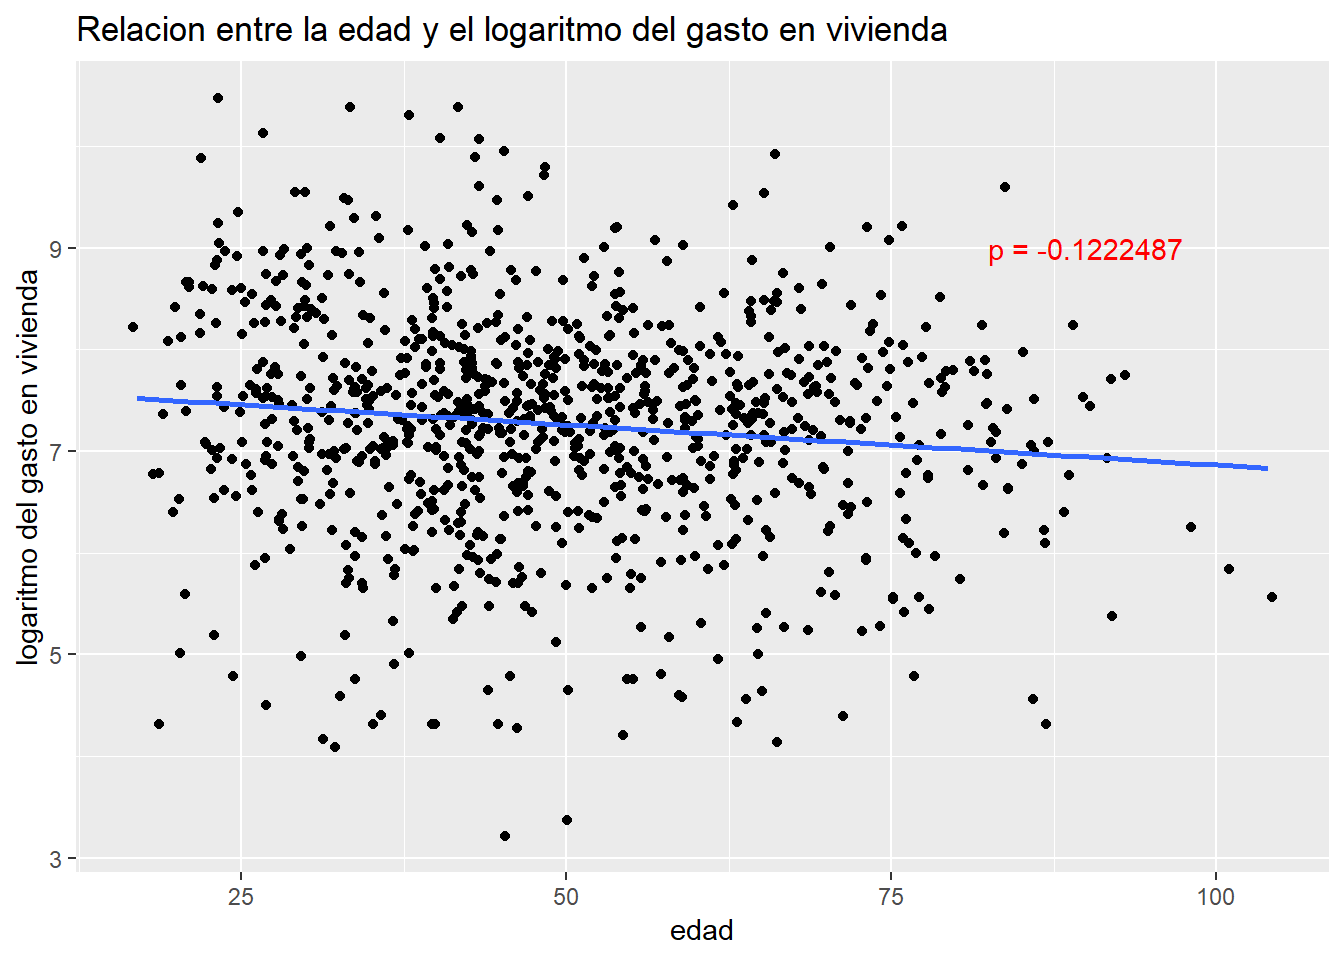
\includegraphics{bookdown-demo_files/figure-latex/unnamed-chunk-23-1.pdf}
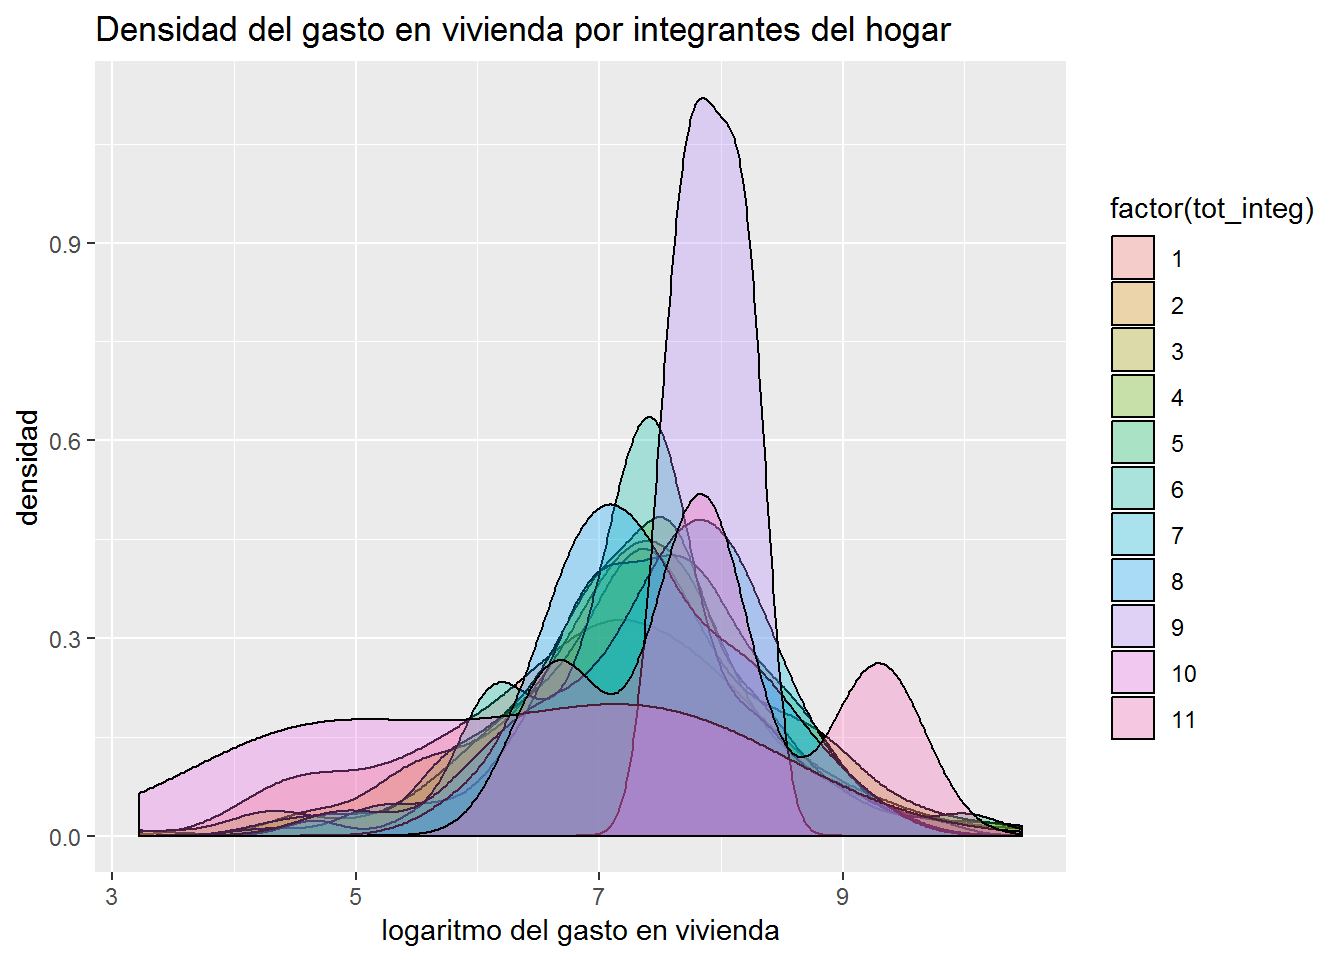
\includegraphics{bookdown-demo_files/figure-latex/unnamed-chunk-23-2.pdf}

\subsubsection{Distribucion del gasto en vivienda agrupado por nivel
educativo del jefe de
familia}\label{distribucion-del-gasto-en-vivienda-agrupado-por-nivel-educativo-del-jefe-de-familia}

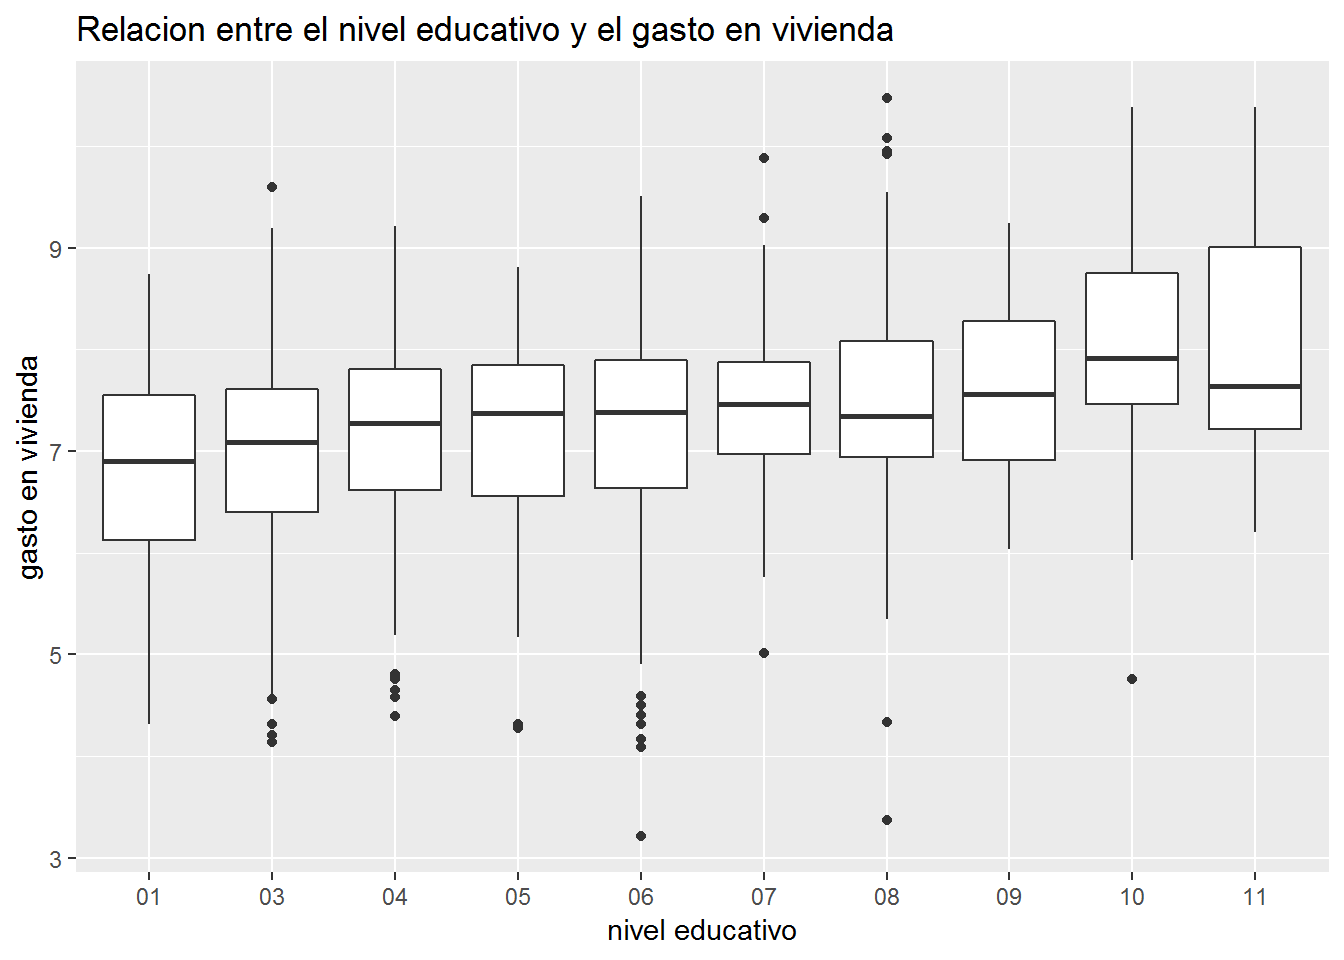
\includegraphics{bookdown-demo_files/figure-latex/unnamed-chunk-24-1.pdf}
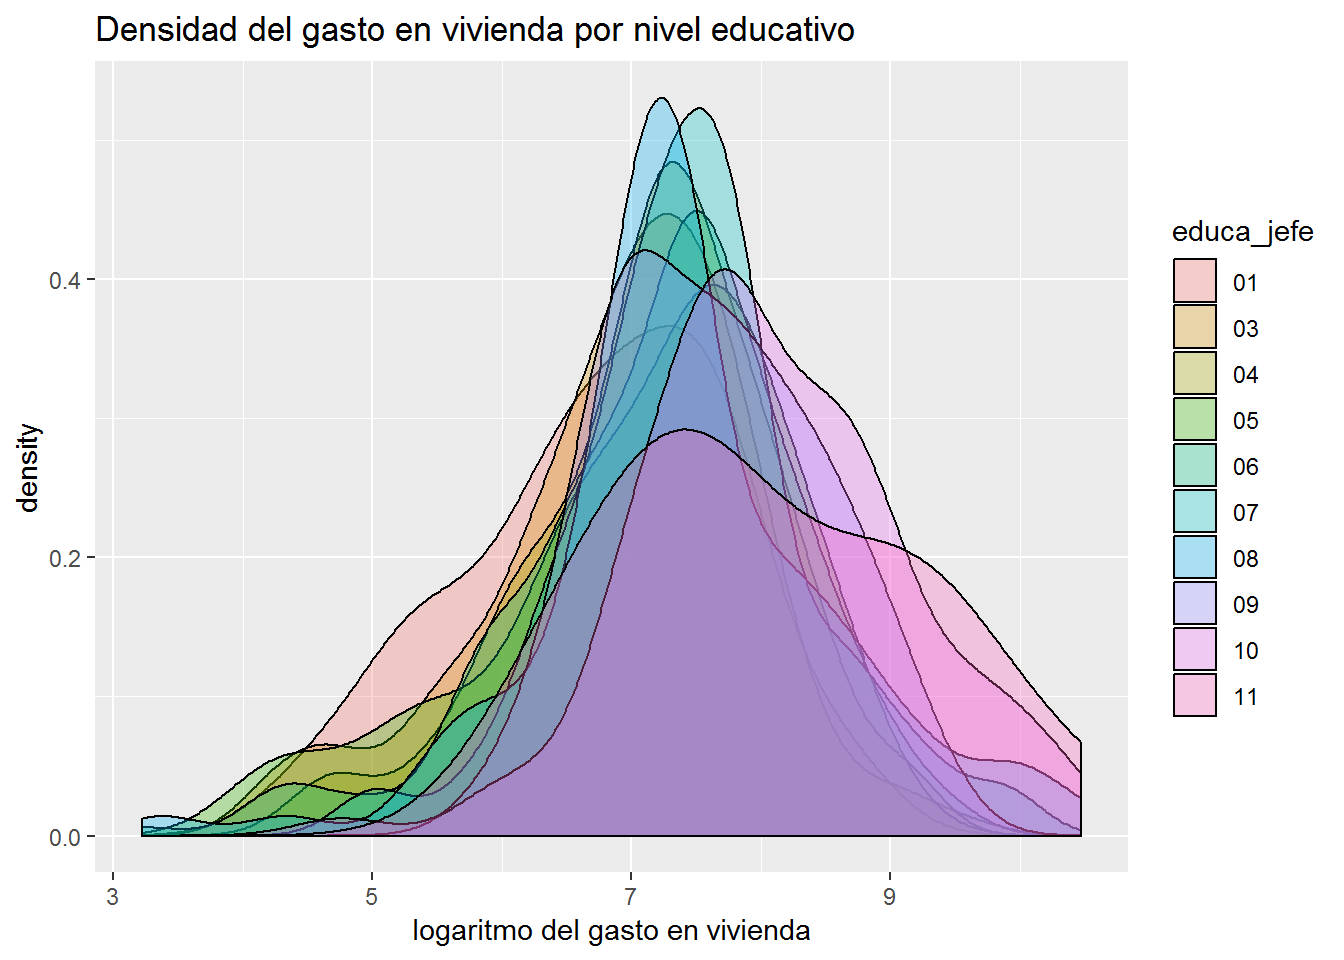
\includegraphics{bookdown-demo_files/figure-latex/unnamed-chunk-24-2.pdf}

\subsubsection{Distribucion del gasto en vivienda agrupado por estrato
socio-economico}\label{distribucion-del-gasto-en-vivienda-agrupado-por-estrato-socio-economico}

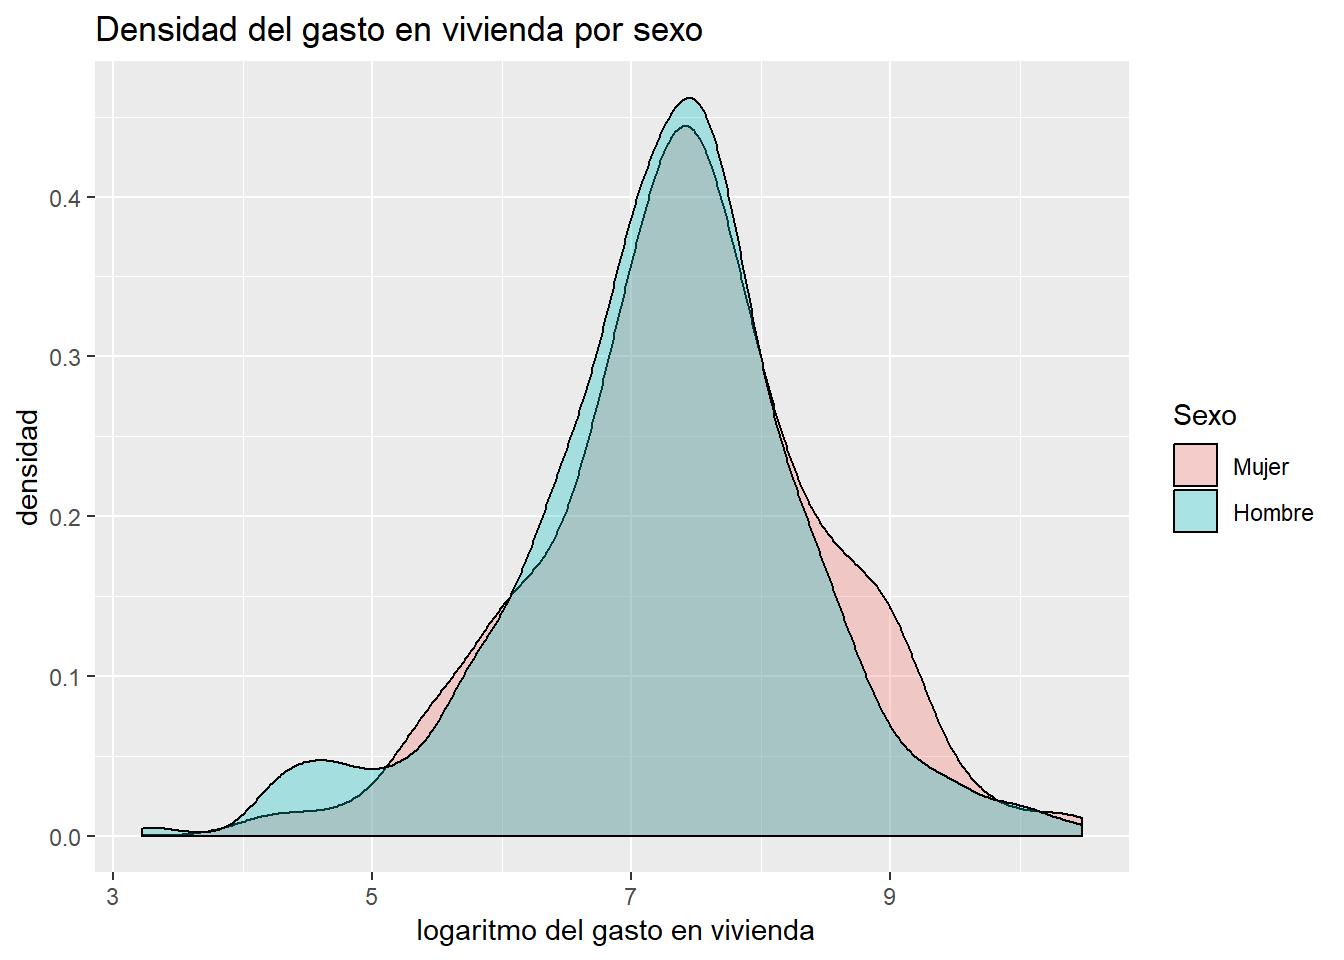
\includegraphics{bookdown-demo_files/figure-latex/unnamed-chunk-25-1.pdf}
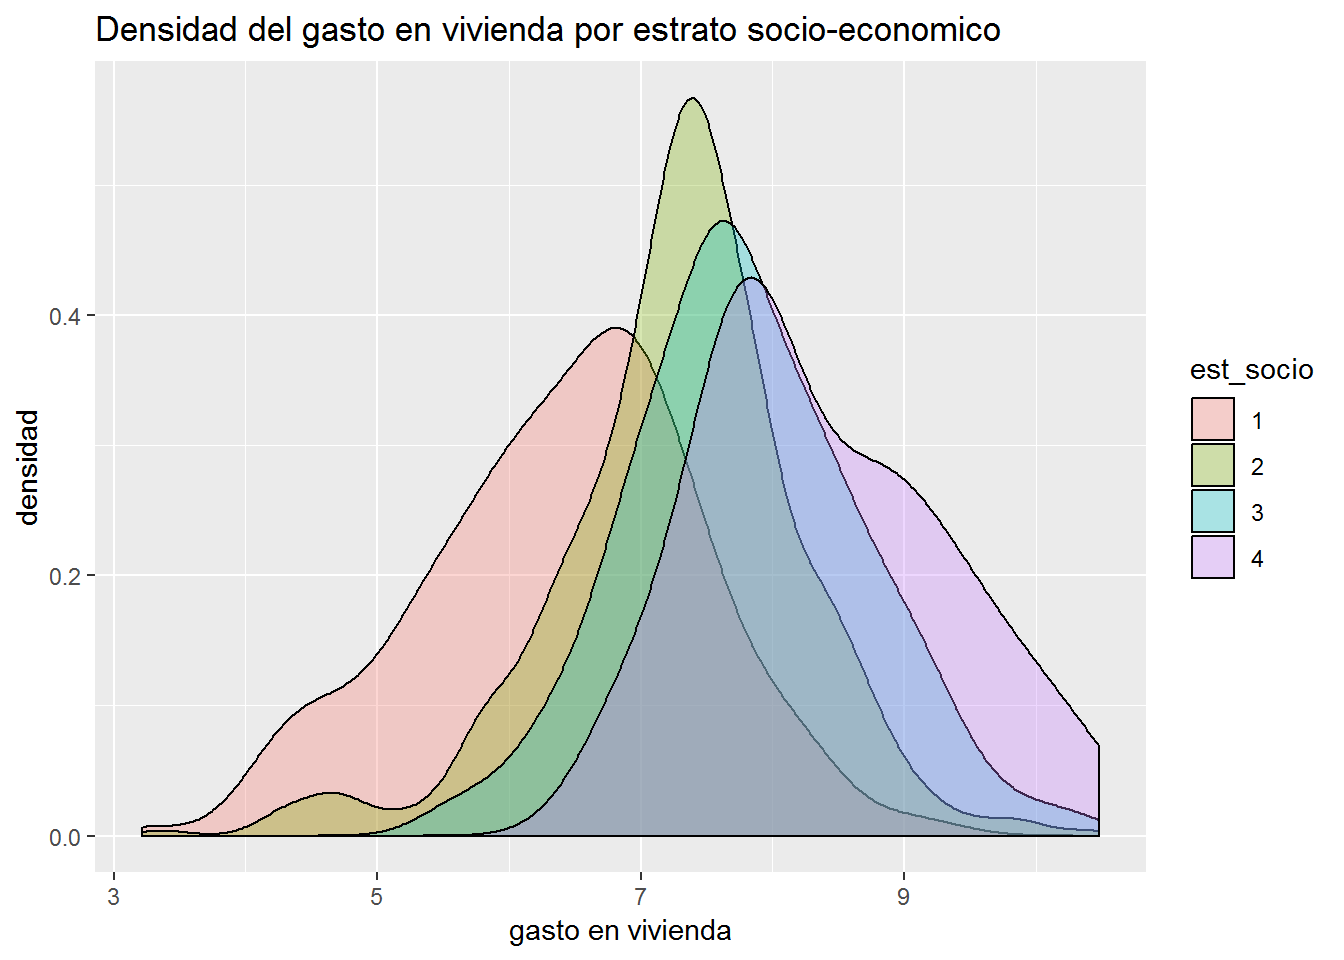
\includegraphics{bookdown-demo_files/figure-latex/unnamed-chunk-25-2.pdf}

\section{Conclusiones del analisis exploratorio de de
datos}\label{conclusiones-del-analisis-exploratorio-de-de-datos}

\begin{itemize}
\tightlist
\item
  Todas las variables numericas en escala logaratmica que componen el
  estudio presentan evidencia de ser distribuidas de forma unimodal y
  simetrica.
\item
  Existen mas hombres jefes de familia que mujeres
\item
  Los hombres asumen la jefatura de la familia a edades menores
\item
  El estrato socio economico mas comun al que pertenecen las familias
  mexicanas es el de Medio-Bajo sin distincion en el sexo del jefe de
  familia.
\item
  El nivel de instruccion formal mas comun de un jefe de familia
  perteneciente al sexo masculino es el de secundaria completa. En caso
  de que el jefe de familia pertenezca al sexo femenino el grado de
  instruccion mas comun es el de primaria completa.
\item
  Mas del 50\% de las personas en el estrato socio-economico bajo tienen
  instruccion formal entre ``sin instruccion'' y ``primaria completa''.
\item
  Mas del 50\% de la personas en el estrato socio economico alto tienen
  estudios de entre profesional completa y posgrado
\item
  La relacion entre el logaritmo del ingreso y el logaritmo del gasto en
  vivienda es lineal, positiva y moderadamente correlacionada.
\item
  La relacion entre el logaritmo del gasto general y el logaritmo del
  gasto en vivienda es lineal, positivo y moderadamente correlacionado.
\item
  La relacion entre la edad y el logaritmo del gasto en vivienda es
  lineal, negativa y debilmente correlacionada.
\item
  No hay evidencia de existir relacion alguna entre el gasto en vivienda
  y los integrantes del hogar.
\item
  No hay evidencia de la existencia de relacion alguna entre el gasto en
  vivienda y el nivel educativo del jefe de familia
\item
  Existe evidencia suficiente que apoye la relacion positiva entre el
  gasto en vivienda y el estrato socio economico al que pertenece una
  familia mexicana.
\end{itemize}

\chapter{Modelo econometrico}\label{modelo-econometrico}

El modelo econometrico que propongo es un modelo lineal generalizado,
cuya variable respuesta se encuentra en escala logaritmica y que puede
ser descrito con la siguiente exucacion :\\
\[\ln(y) = \beta_{0} + \beta_{1}x_{1} + \beta_{2}x_{2} + \beta_{3}x_{3} + \beta_{4}x_{4} + \beta_{5}x_{5} +  \beta_{6}x_{6} + \beta_{7}x_{7} + \epsilon \]

Donde:\\
\(\ x_{1}\) Es esl gasto general trimestral reportado por la unidad de
observaci?n medido en escala logaritmica.\\
\(\ x_{2}\) Es la edad del jefe de familia.\\
\(\ x_{3}\) Es la edad del jefe de familia al cuadrado.\\
\(\ x_{4}\) Es que el sexo del jefe de familia es masculino.\\
\(\ x_{5}\) La unidad de an?lisis pertenece al estrato socio economico
2.\\
\(\ x_{6}\) La unidad de analisis pertenece al estrato socio economico
3.\\
\(\ x_{7}\) La unidad de analisis pertenece al estrato socio economico
4.

\section{Resultados del modelo de
regresion}\label{resultados-del-modelo-de-regresion}

\begin{verbatim}
## 
## Call:
## lm(formula = log(vivienda) ~ log(gasto_mon) + edad_jefe + I(edad_jefe^2) + 
##     sexo_jefe + est_socio, data = datos2)
## 
## Residuals:
##     Min      1Q  Median      3Q     Max 
## -3.2057 -0.5016  0.0397  0.5480  2.2927 
## 
## Coefficients:
##                  Estimate Std. Error t value Pr(>|t|)    
## (Intercept)     1.336e+00  4.186e-01   3.191  0.00146 ** 
## log(gasto_mon)  6.602e-01  3.904e-02  16.912  < 2e-16 ***
## edad_jefe      -4.155e-02  8.802e-03  -4.720 2.70e-06 ***
## I(edad_jefe^2)  3.897e-04  8.278e-05   4.708 2.87e-06 ***
## sexo_jefe1     -2.055e-01  6.247e-02  -3.289  0.00104 ** 
## est_socio2      5.864e-01  7.197e-02   8.147 1.15e-15 ***
## est_socio3      8.707e-01  9.115e-02   9.553  < 2e-16 ***
## est_socio4      1.133e+00  1.361e-01   8.320 3.00e-16 ***
## ---
## Signif. codes:  0 '***' 0.001 '**' 0.01 '*' 0.05 '.' 0.1 ' ' 1
## 
## Residual standard error: 0.8268 on 961 degrees of freedom
## Multiple R-squared:  0.4188, Adjusted R-squared:  0.4146 
## F-statistic: 98.94 on 7 and 961 DF,  p-value: < 2.2e-16
\end{verbatim}

\begin{verbatim}
## Analysis of Variance Table
## 
## Response: log(vivienda)
##                 Df Sum Sq Mean Sq  F value    Pr(>F)    
## log(gasto_mon)   1 363.78  363.78 532.1165 < 2.2e-16 ***
## edad_jefe        1   0.64    0.64   0.9384    0.3329    
## I(edad_jefe^2)   1  15.10   15.10  22.0924 2.978e-06 ***
## sexo_jefe        1  14.37   14.37  21.0195 5.146e-06 ***
## est_socio        3  79.58   26.53  38.8010 < 2.2e-16 ***
## Residuals      961 656.99    0.68                       
## ---
## Signif. codes:  0 '***' 0.001 '**' 0.01 '*' 0.05 '.' 0.1 ' ' 1
\end{verbatim}

\begin{verbatim}
##                        2.5 %        97.5 %
## (Intercept)     0.5143712362  2.1572688403
## log(gasto_mon)  0.5835896271  0.7368019585
## edad_jefe      -0.0588241483 -0.0242766405
## I(edad_jefe^2)  0.0002272565  0.0005521679
## sexo_jefe1     -0.3280454049 -0.0828596406
## est_socio2      0.4451288375  0.7276122742
## est_socio3      0.6918135486  1.0495494610
## est_socio4      0.8654571212  1.3997876225
\end{verbatim}

\subsection{Interpretacion de los resultados de
regresion}\label{interpretacion-de-los-resultados-de-regresion}

Despues de ajustar el modelo con los regresores propuestos, podemos
escribir la ecuacion de regresion como:

\[\ \hat{ln(y)} = 1.336 + 0.6602x_{2} - 0.04155x_{2} + 0.0003897x_{3} -0.255x_{4} + 0.5864x_{5} + 0.8707x_{6} + 1.133x_{7}\]

El P-value de la prueba F de significancia global del modelo esta por
debajo del \(\alpha\) = 0.05 (numero que, generalmente se utiliza para
evaluar la significancia de pruebas estad?sticas), recordemos que la
hipotesis a contrastar en la prueba de significancia global son
\[ \ H_{0} : \beta_{1} = \beta_{2} = \cdots = \beta_{7} = 0 \hspace{0.5cm}vs.\hspace{0.5cm} H_{1} : \exists \hspace{0.3cm}   \beta_{i} \neq 0 \hspace{0.3cm} \ p.a  \hspace{0.3cm} \ i \hspace{0.3cm} \epsilon  \hspace{0.3cm} \{1,2,\dots,7\} \]
Del resultado de la prueba, rechazao la hipotesis nula, por lo que
alguno de los coeficientes de mi modelo es distinto de cero, y por lo
tanto el modelo es globalmente significativo.

El P-value de las pruebas t de significancia individual de todos los
parametros esta por debajo del \(\alpha = 0.05\) ,por lo que rechazo la
hipotesis nula, recordemos que las hipotesis a contrastar de la prueba t
de significancia indivual es :
\[ \ H_{0}:\frac{\hat{\beta_{j}}}{S(\beta_{j})} = 0 \hspace{0.5cm} vs \hspace{0.5cm} H_{1} : \frac{\hat{\beta_{j}}}{S(\hat{\beta_{j}})} \neq 0\]
Por lo que todas las variables incluidas en el modelo tienen algún
(\textbf{Caeteris Paribus}) sobre el gasto en vivienda que no es debido
solamente al azar de tal forma que son estadisticamente significativas.

Puedo decir que, de acuerdo a la medida de bondad de ajuste \(\ R^{2}\)
ajustado que 41\% de la desviacion del modelo base es directamente
imputable a la existencia de correlacion de la variable explicada con
los regresores.

El modelo base es aquel donde solo se tienen en cuenta los efectos
capturados por el intercepto al origen (\(\hat{\beta_{0}}\)), es decir,
cuando el resto de las \$~x\_\{i\} \$ se mantienen en 0.

Las unidades observacionales que no cumplen explicitamenente alguna de
las caracteristicas de las variables categericas( por ejemplo, que el
sexo del jefe de familia sea femenino, o que la familia pertenezca al
estrato socio-economico 1) son efectos capturados en el modelo base

\section{Analisis de residuales}\label{analisis-de-residuales}

El analisis de residuales es una herramienta que me ayudara a comprobar
los supuestos que todo modelo de regresion lineal multiple
(\textbf{RLM}) debe cumplir, esto para saber que la inferencia sobre los
parametros del modelo es correcta y confiable. Los supuestos de
\textbf{RLM} son:

\textbf{Independencia de los errores}
\[ \ F_{\epsilon_{1},\epsilon_{2}\dots,\epsilon_{n}}(\epsilon_{1},\epsilon_{2},\dots,\epsilon_{n}) = F_{\epsilon_{1}}(\epsilon_{1}) F_{\epsilon_{2}}(\epsilon_{2})\dots  F_{\epsilon_{n}}(\epsilon_{n}) \]
donde F es la funcion de distribucion de las perturbaciones.

\begin{enumerate}
\def\labelenumi{\arabic{enumi}.}
\item
  \textbf{Linealidad en los parametros} : para cualquier combinacion de
  los valores de \(\ x_{i}\) se tiene que:\\
  \[ \ E(\hat{\epsilon}|X) = 0 \] Esto es para que los estimadores de
  los efectos ceteris paribus sean insesgados
\item
  \textbf{Homocedasticidad condicional} : La varianza de los residuos,
  dados los parametros es constante, i.e:
\end{enumerate}

\[ \ Var(\hat{\epsilon_{i}}|X) = \sigma_{\epsilon}^{2} \]

\begin{enumerate}
\def\labelenumi{\arabic{enumi}.}
\setcounter{enumi}{2}
\tightlist
\item
  \textbf{Normalidad multivariada} : Los residuos se distribuyen normal
  con media 0 y varianza constante, i.e:
\end{enumerate}

\[ \hat{\epsilon}  \sim {\sf }N(0,\sigma_{\epsilon}^{2}) \] Esto es para
que los estimadores de los coeficientes de regresion sean eficientes (de
minima varianza) y que los intervalos de confianza sean exactos.

\begin{enumerate}
\def\labelenumi{\arabic{enumi}.}
\setcounter{enumi}{3}
\tightlist
\item
  \textbf{No existencia de multicolinealidad perfecta} : Ninguna de las
  columnas de la matriz \(\ X\) (la matriz de diseno) es combinacion
  lineal del resto de las columnas, esto es: \[ \ |(X^{T}X)^{-1}| > 0 \]
  Esto se pide para que sea posible calcular los estimadores de los
  coeficientes de regresion, sin empargo, la \textbf{Multicolinealidad
  imperfecta} que es: \[ \ |(X^{T}X)^{-1}| \approx 0 \] que se presenta
  cuando existe una alta correlacion entre variables tambien representa
  un grave error en un modelo, ya que se ``inflan'' los errores estandar
  de los estimadores, lo cual genera una impresicion y
  ``ensanchamiento'' de los intervalos de confianza.
\end{enumerate}

\subsection{Tests graficos para comprobar los supuestos de regresion
lineal
multiple}\label{tests-graficos-para-comprobar-los-supuestos-de-regresion-lineal-multiple}

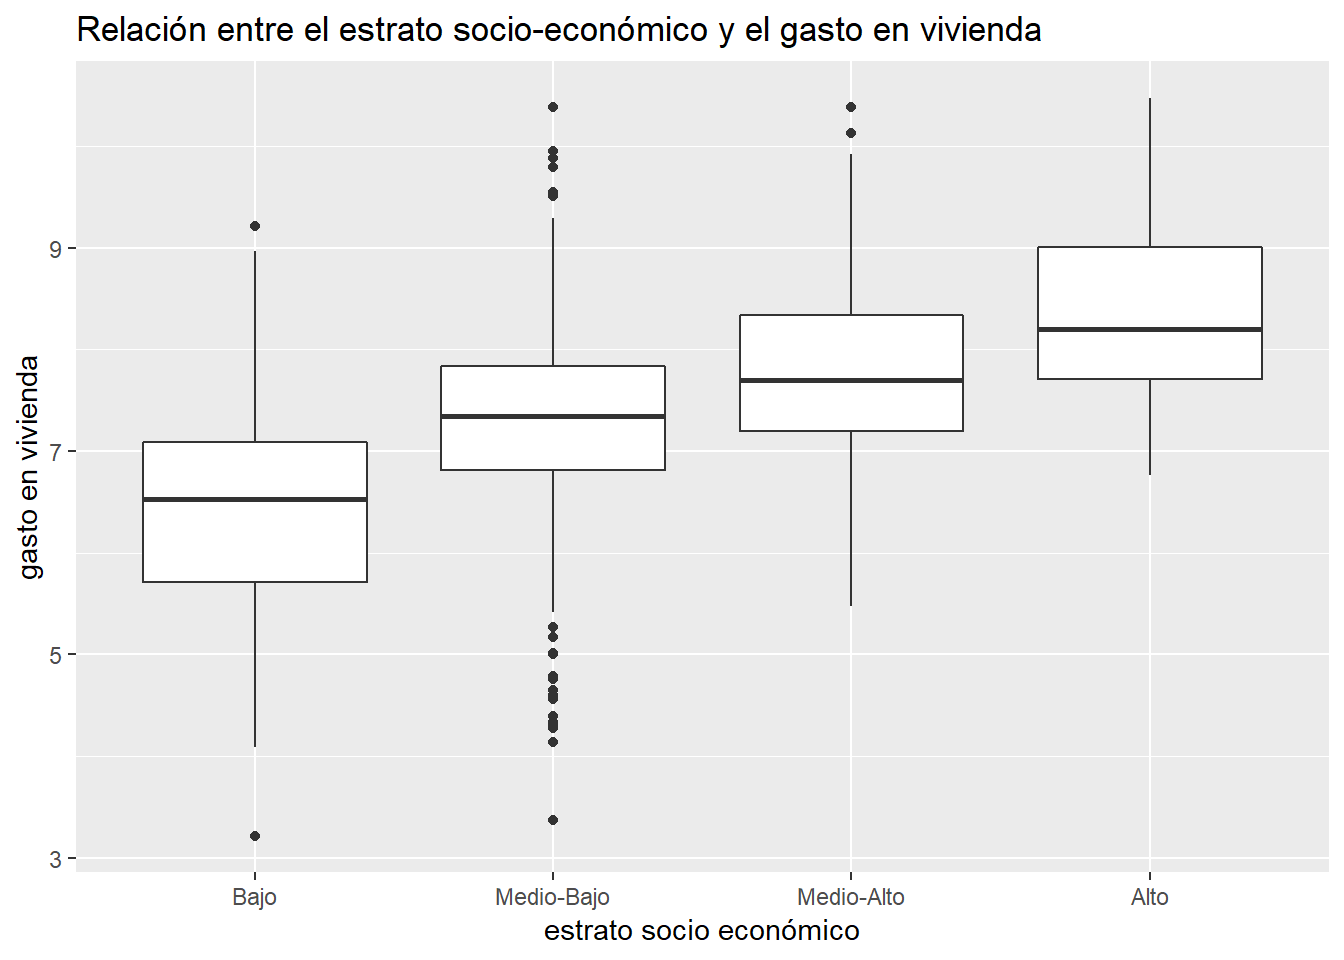
\includegraphics{bookdown-demo_files/figure-latex/unnamed-chunk-30-1.pdf}

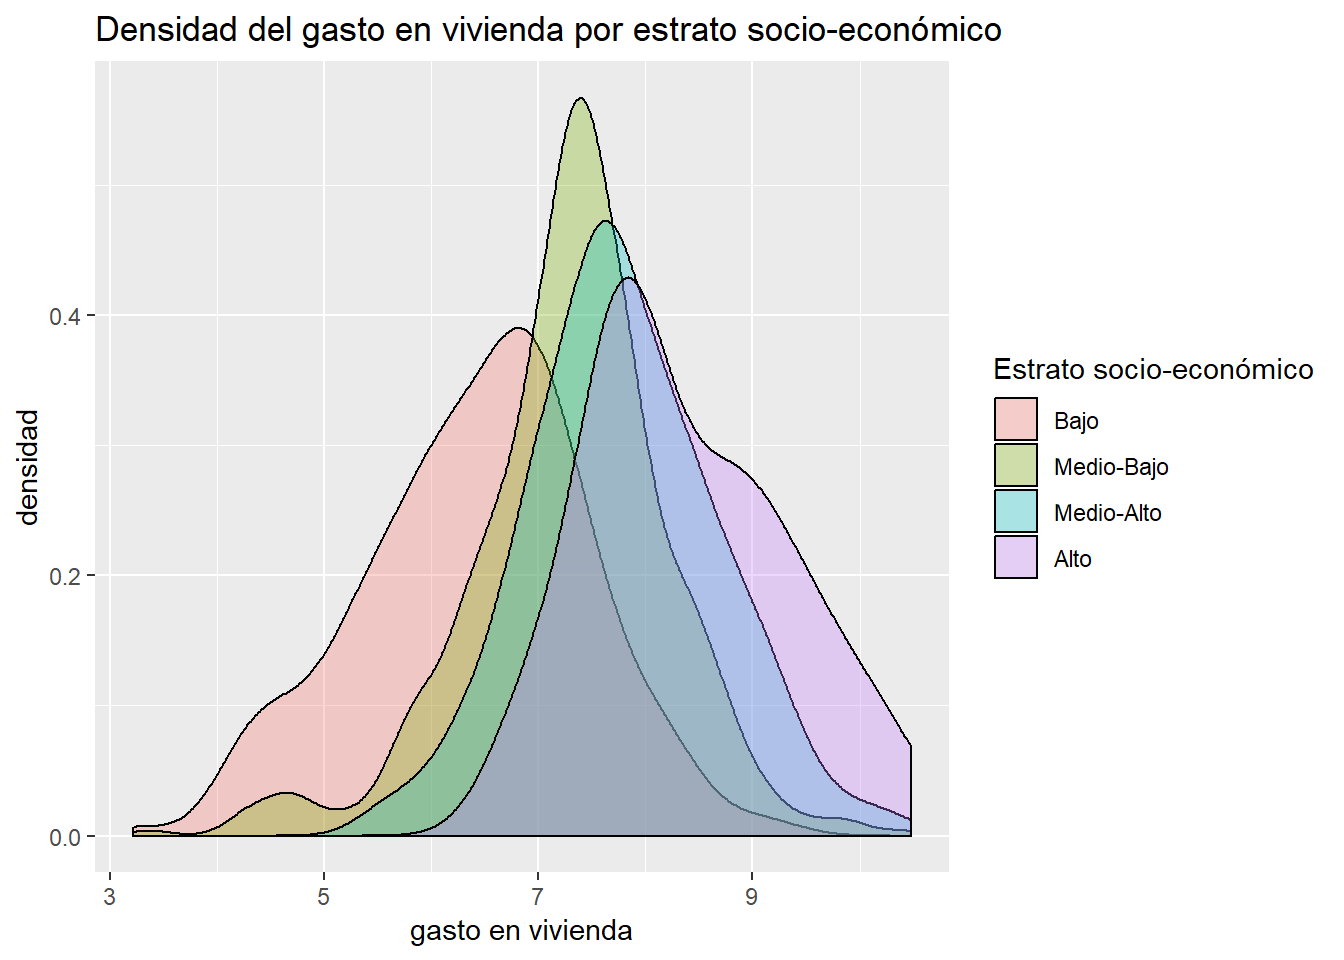
\includegraphics{bookdown-demo_files/figure-latex/unnamed-chunk-31-1.pdf}

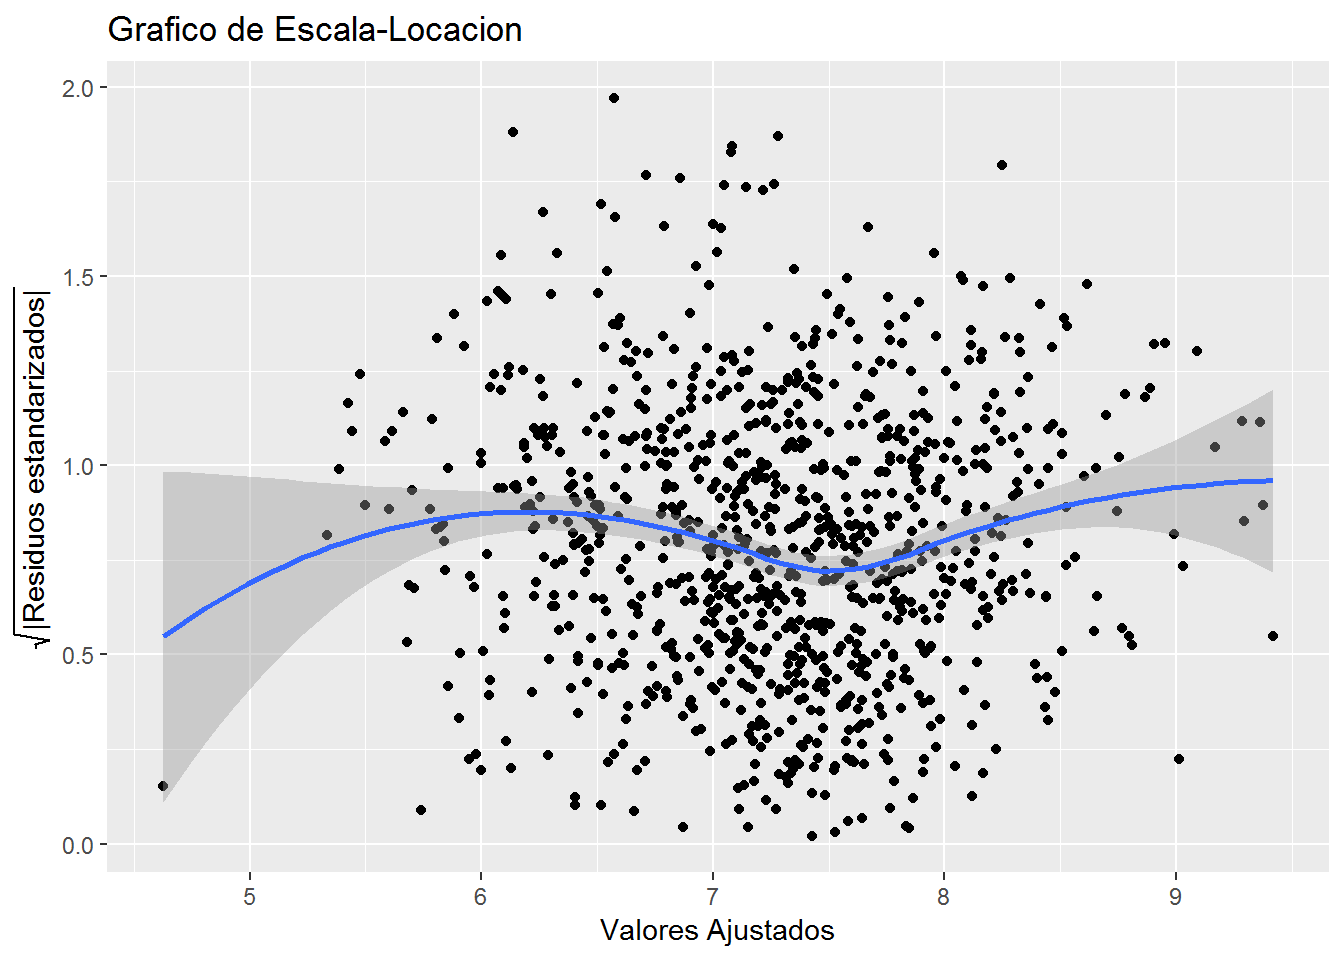
\includegraphics{bookdown-demo_files/figure-latex/unnamed-chunk-32-1.pdf}

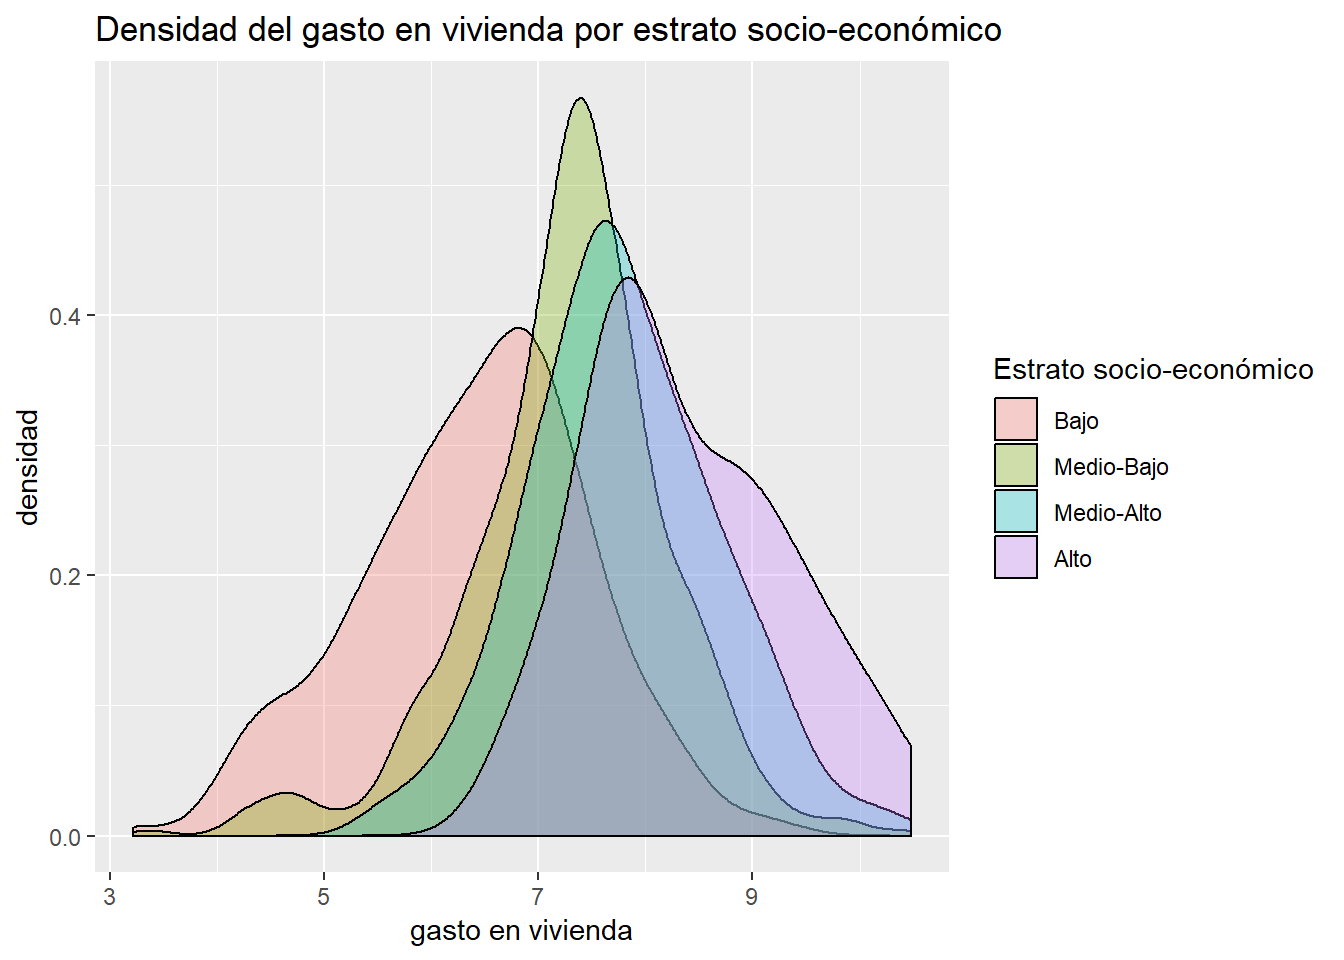
\includegraphics{bookdown-demo_files/figure-latex/unnamed-chunk-33-1.pdf}

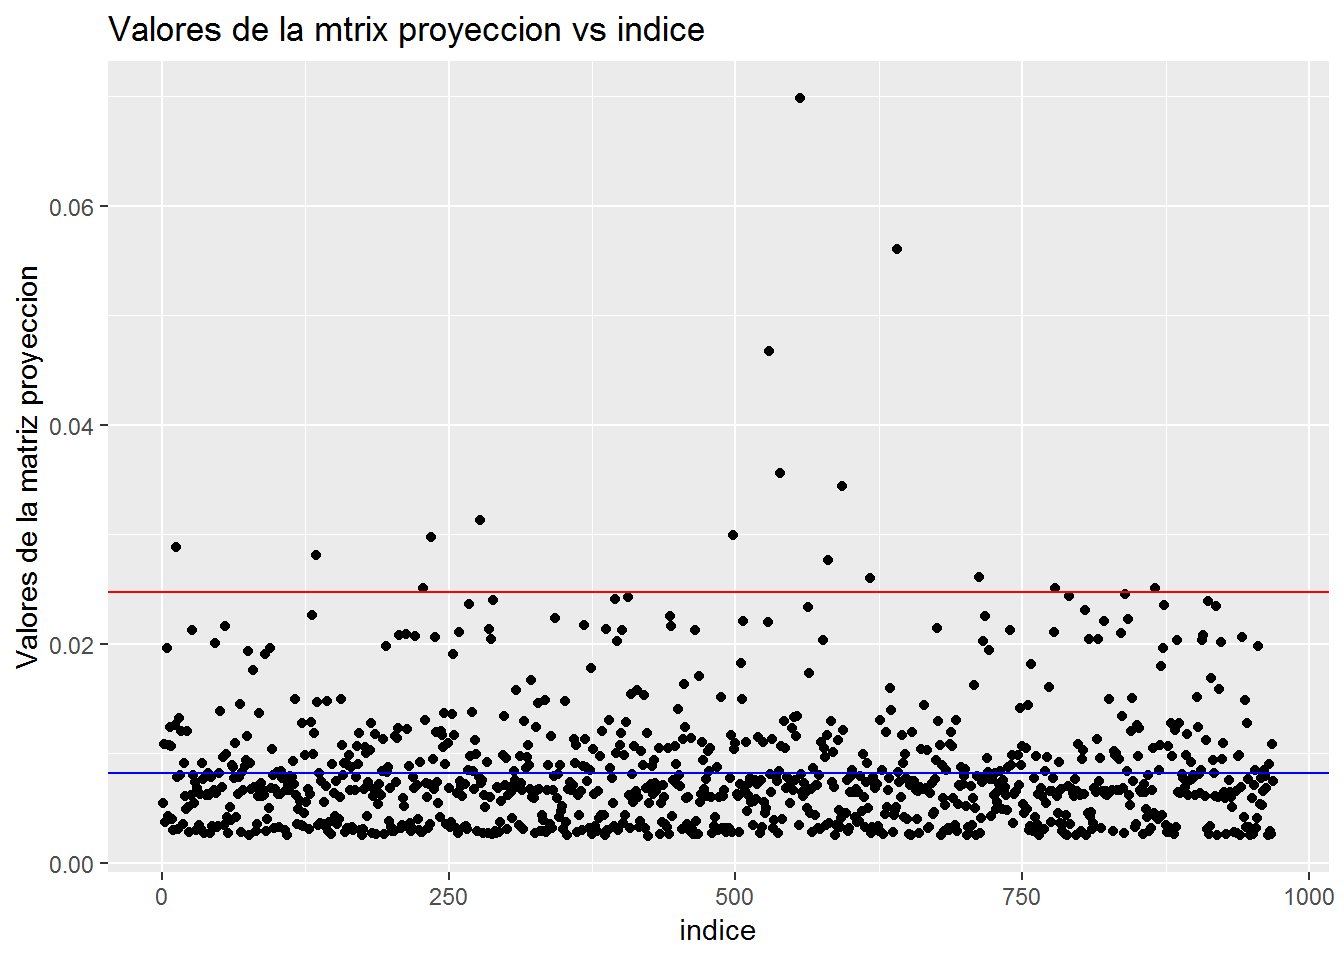
\includegraphics{bookdown-demo_files/figure-latex/unnamed-chunk-34-1.pdf}

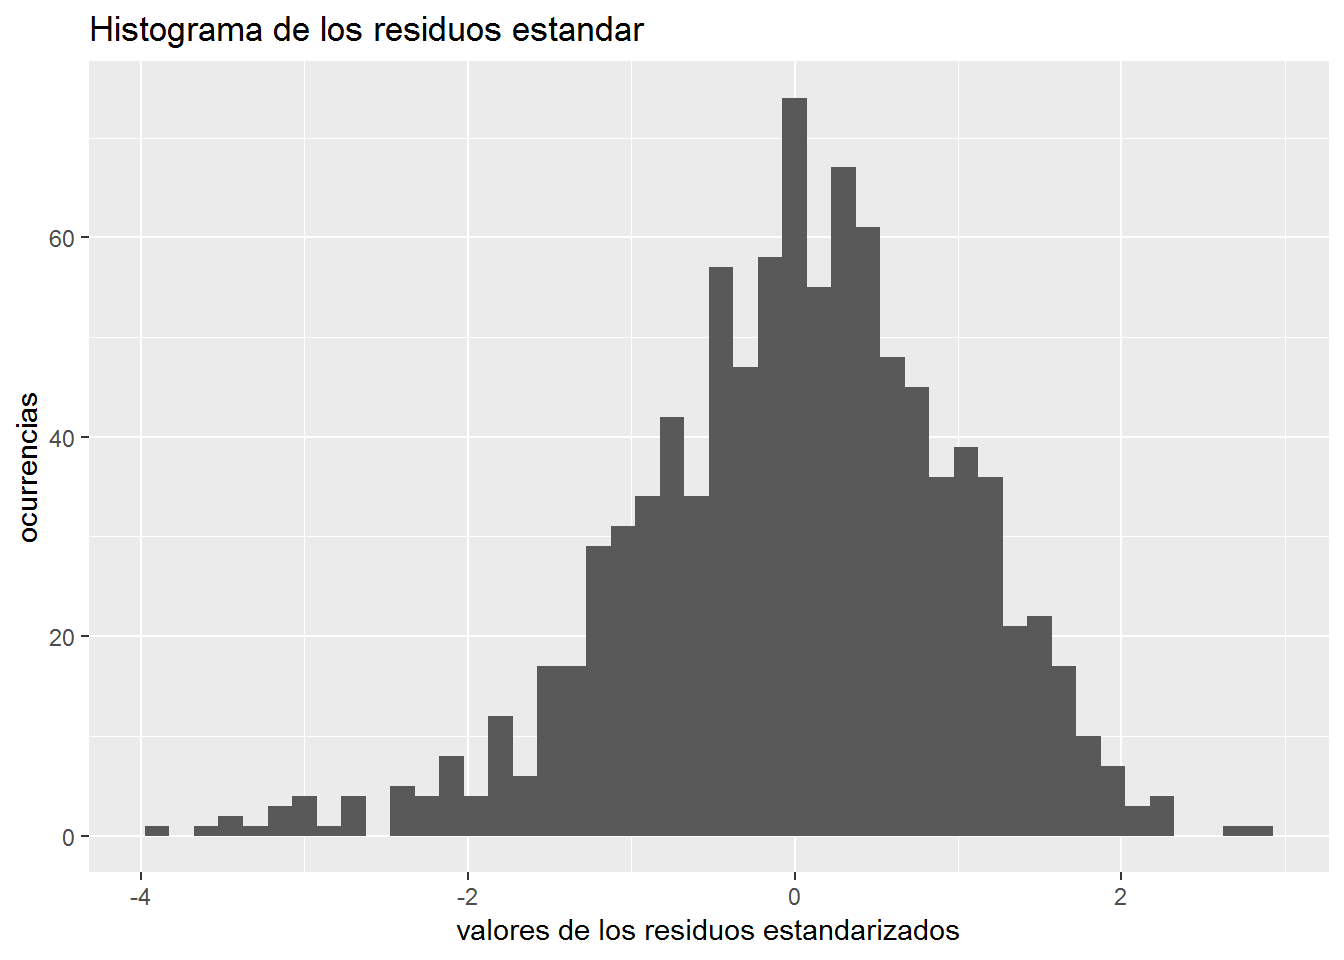
\includegraphics{bookdown-demo_files/figure-latex/unnamed-chunk-35-1.pdf}

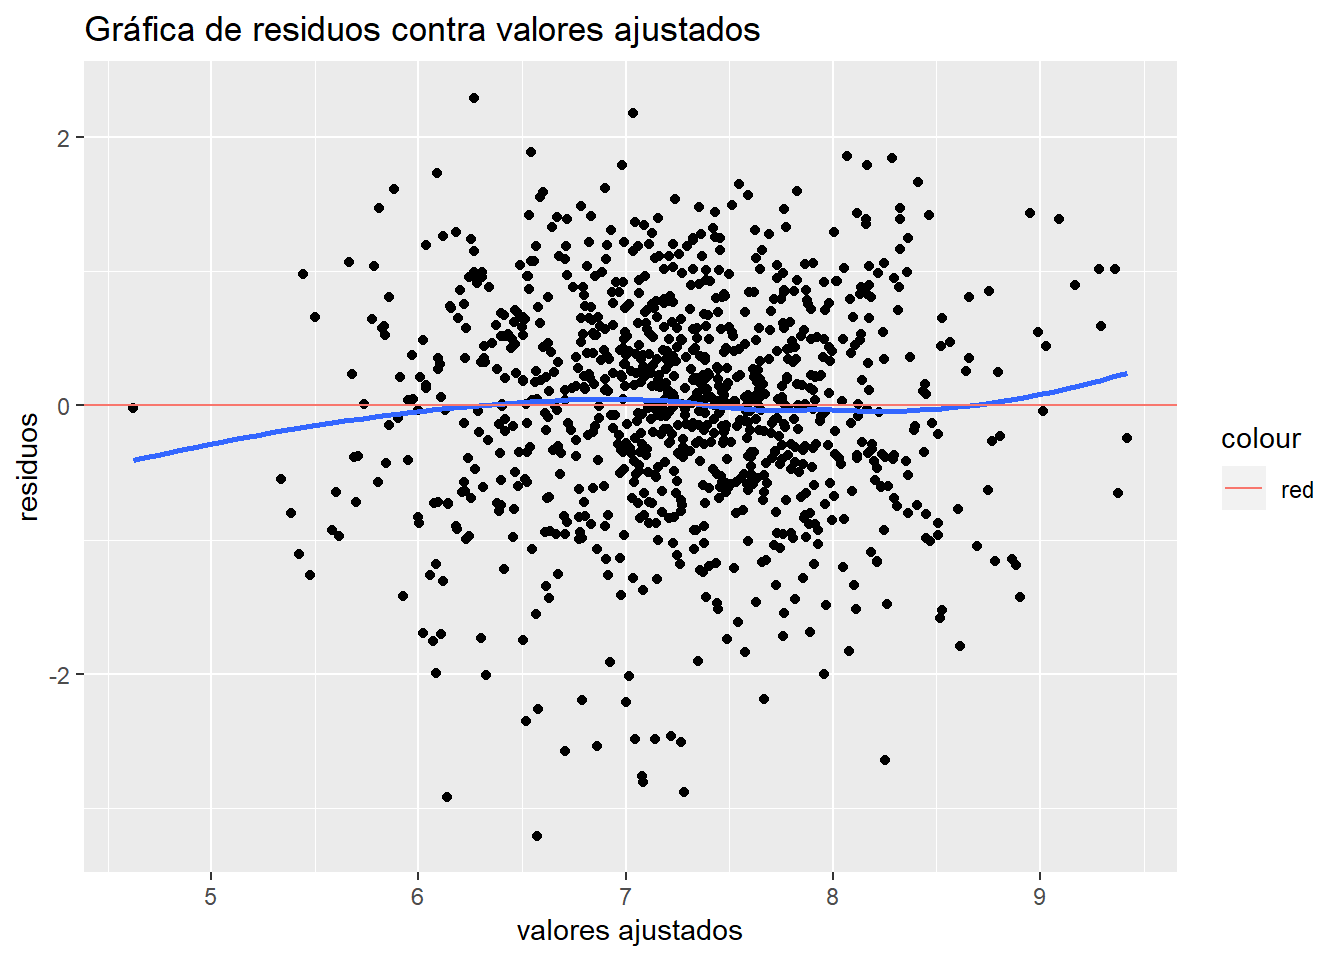
\includegraphics{bookdown-demo_files/figure-latex/unnamed-chunk-36-1.pdf}

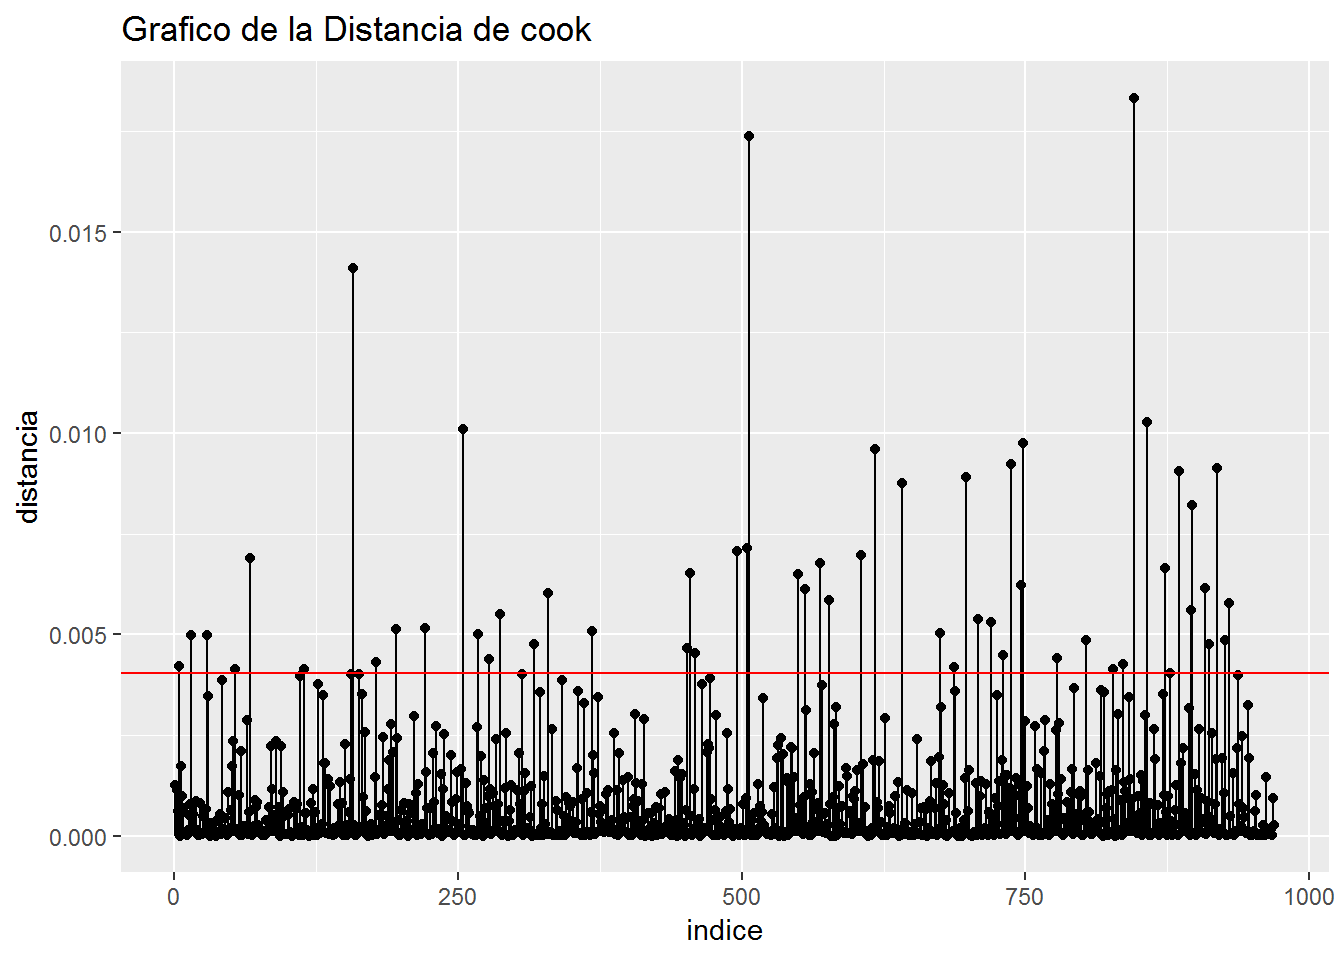
\includegraphics{bookdown-demo_files/figure-latex/unnamed-chunk-37-1.pdf}

\subsection{Tests estadisticos para comprobar las hipotesis de regresion
lineal
multiple}\label{tests-estadisticos-para-comprobar-las-hipotesis-de-regresion-lineal-multiple}

Quiero comprobar que la esperanza de los residuos sea 0 , por lo que
hare el siguiente contraste de hipotesis con una prueba t
\[ \ H_{0} : E(\epsilon|X) = 0 \hspace{0.5cm} vs \hspace{0.5cm} H_{1}: E(\epsilon|X) \neq 0 \]

\begin{verbatim}
## [1] 1
\end{verbatim}

Como el P-value es mayor que el valor de significancia \$ \alpha = 0.05
\$ acepto la hipotesis nula de que los residuos tienen valor esperado 0.

Aplico la prueba de Durbin-Watson para detectar si el coeficiente de
correlacion es 0 o distinto de cero, esto para verificar la
independencia de los residuos, sus hipotesis son :

\[ \ H_{0} : \rho(i,i+1) = 0 \hspace{0.5cm} vs \hspace{0.5cm} H_{1}: \rho(i,i+1) \neq 0 \]

\begin{verbatim}
##  lag Autocorrelation D-W Statistic p-value
##    1      0.01480526      1.968207    0.66
##  Alternative hypothesis: rho != 0
\end{verbatim}

Como el P-value es mayor que el valor \$ \alpha = 0.05\$ entonces acepto
la hipotesis nula de que el coeficiente de correlacion es 0.

Aplico la prueba de Breusch-Pagan, cuyas hipotesis a contrastar son : La
varianza de los residuos es constante vs.~la varianza de los residuos es
una funcion de los valores ajustados del modelo. Esto es para verificar
la homocedasticidad.
\[ \ H_{0}: Var(\hat{\epsilon} |X) = \sigma_{\epsilon}^{2} \hspace{0.5cm} vs \hspace{0.5cm} H_{1}: Var(\hat{\epsilon} |X) =  \sigma_{\epsilon}^{2}( \hat{Y}) \]

\begin{verbatim}
## 
##  studentized Breusch-Pagan test
## 
## data:  fitb
## BP = 5.9653, df = 7, p-value = 0.5438
\end{verbatim}

Como el P-value es mayor que \$ \alpha = 0.05\$ , por lo tanto acepto la
hipotesis nula de una varianza constante.

Tambien proveo el resultado de la prueba de Goldfeld-Quandt, cuyas
hipotesis son: La varianza es igual en un primer grupo de residuos que
en un segundo grupo de residuos vs, la varianza en el primer grupo de
residuo es es menor que la varianza en un segundo grupo (es decir, la
varianza aumenta conforme crecen los valores ajustados del modelo) h
\[ \ H_{0}: \sigma_{\epsilon_{1}}^{2} = \sigma_{\epsilon_{2}}^{2} \hspace{0.5cm} vs   \hspace{0.5cm} H_{1}: \sigma_{\epsilon_{1}}^{2} < \sigma_{\epsilon_{2}}^{2}\]

\begin{verbatim}
## 
##  Goldfeld-Quandt test
## 
## data:  fitb
## GQ = 0.58906, df1 = 477, df2 = 476, p-value = 1
## alternative hypothesis: variance increases from segment 1 to 2
\end{verbatim}

Como el P-value es mayor que el valor de significancia \$ \alpha =
0.05\$ entonces acepto la hipotesis nula de que la varianza es igual en
ambos segmentos

Proveo tambien el resultado de la prueba de Kolmogorov-Smirnov, cuyas
hipotesis a contrastar son :

\[ H_{0}: \frac{\hat{\epsilon}}{\sqrt{S^{2}(1-h_{i})}} \sim N(0,1) \hspace{0.5cm} vs \hspace{0.5cm} \frac{\hat{\epsilon}}{\sqrt{S^{2}(1-h_{i})}} \nsim N(0,1) \hspace{0.5cm}  \]

\begin{verbatim}
## 
##  One-sample Kolmogorov-Smirnov test
## 
## data:  resultados_fit$.std.resid
## D = 0.037732, p-value = 0.1267
## alternative hypothesis: two-sided
\end{verbatim}

Como el P-value es mayor que el valor de significancia \$ \alpha =
0.05\$ entonces acepto la hipotesis nula de que los residuos
estandarizados se distribuyan normal con parametros de media 0 y
varianza 1.

La identificacion de la multicolinealidad no se puede hacer de forma
tradicional en este modelo, ya que se incluye un termino cuadratico (la
edad del jefe de familia al cuadrado) como regresor, por lo cual, para
proveer evidencia de que no existe multicolinealidad entre los
regresores, cree un modelo de regresion auxiliar donde excluyo el
termino cuadratico. A continuacion presento los factores de inflacion de
varianza (FIV) de esa regresion auxiliar.

Recordemos que los FIV se calculan en dos pasos, primero se crean i
distintas regresiones por el m?todo de m?nimos cuadrados cuya variable
explicada es \(\ X_{i}\) y los regresores son el resto de las variables,
es decir

\[ \ x_{i} = \alpha_{0} + \alpha_{1}x_{1} + \dots + \alpha_{k}x_{k} + \epsilon \]
Despues se calcula el FIV para cada coeficiente \(\hat{\beta_{i}}\) del
modelo de regresion original (En nuestro caso es el modelo que no
incluye el termino cuadratico) \[ \ FIV_{i} = \frac{1}{1-R^{2}_{i}} \]
Donde \(\ R_{i}^{2}\) es el coeficiente de determinacion de la regresion
cuya variable explicada es \$ \x\_\{i\}\$ y sus regresores son el resto
de las k variables explicativas.

Por lo general se dice que una variable aporta colinealidad al modelo si
\(\ FIV(\hat{\beta_{i}}) > 10\) lo cual claramente no ocurre entre los
regresores, por lo que podemos descartar la existencia de
multicolinealidad ya que no existe evidencia suficiente en pro de esta.

\begin{verbatim}
##                    GVIF Df GVIF^(1/(2*Df))
## log(gasto_mon) 1.296543  1        1.138658
## edad_jefe      1.090427  1        1.044235
## sexo_jefe      1.037531  1        1.018593
## est_socio      1.226484  3        1.034611
\end{verbatim}

\subsection{Identificacion de los valores extremos e
influyentes}\label{identificacion-de-los-valores-extremos-e-influyentes}

A continuacion presento una tabla cuyos metricas de residuo estandar y
distancia de cook son aparentemente mas grandes que el resto (residuo
estandar \textgreater{} 3 \& distancia de cook \textgreater{} 4 veces el
promedio de la distancia de cook de los residuos), esto por que son
potenciales observaciones extremas.

\begin{table}

\caption{\label{tab:unnamed-chunk-44}Tabla de los valores influyentes}
\centering
\begin{tabular}[t]{r|r|r}
\hline
count & .std.resid & .cooksd\\
\hline
157 & -3.212012 & 0.0140883\\
\hline
506 & -3.026296 & 0.0173619\\
\hline
569 & -3.494389 & 0.0067647\\
\hline
698 & -3.125113 & 0.0088935\\
\hline
737 & -3.886520 & 0.0092244\\
\hline
846 & -3.098029 & 0.0183249\\
\hline
857 & -3.540299 & 0.0102776\\
\hline
\end{tabular}
\end{table}

\chapter{Interpretacion economica del
modelo}\label{interpretacion-economica-del-modelo}

Segun los resultados del estudio, y manteniendo todo lo demas constante
(\textbf{Ceteris Paribus}) :

\begin{itemize}
\item
  El gasto en vivienda parte de los \$3.8073 pesos.
\item
  Un incremento de un punto porcentual en el gasto, repercute en un
  incremento porcentual del 0.6602\% en el gasto en vivienda, por la
  especificacion del modelo, este tiene una interpretaci?n de
  elasticidad con respecto a esta variable.
\item
  Un incremento en una unidad de edad del jefe de familia representa un
  detrimento del 4.155\% en el gasto en vivienda, pero ya que anadi el
  termino cuadratico a la forma funcional del modelo tambien significa
  un incremento del .03987\% en el gasto en vivienda, esta relacion
  proviene de los rendimientos marginales decrecientes proporcionados
  por la edad.
\item
  El hecho de que el jefe de familia pertenezca al sexo masculino se
  puede traducir en un detrimento del gasto en vivienda de 25.54\%.
\item
  Al pertenecer al estrato socio economico Medio-Bajo el hogar gasta
  58.64\% en vivienda mas en vivienda que las familias que pertenecen al
  estrato socio economico Bajo.
\item
  Al pertenecer al estrato socio-economico Medio-Alto la unidad de
  observacion gasta un 87.07\% mas en vivienda que las familias que
  pertenecen al estrato socio economico Bajo.
\item
  Al pertenecer al estrato socio-economico Alto, la unidad la familia
  gasta un 113.3\% mas en vivienda que las familias que pertenecen al
  estrato socio economico Bajo.
\item
  Para realizar predicciones sobre el gasto en vivienda de una familia
  mexicana, es conveniente regresar a la unidad original, es decir
  expresar la esperanza de Y en pesos en vez de en logaritmos, esto lo
  logramos exponenciando la ecuacion del modelo de ambos lados, de lo
  cual resulta la siguiente ecuaci?n.
\end{itemize}

\[ \ E[Y| X] = e^{1.336 + 0.6602x_{2} - 0.04155x_{2} + 0.0003897x_{3} -0.255x_{4} + 0.5864x_{5} + 0.8707x_{6} + 1.133x_{7}}  \]

\chapter{Evaluacion predictiva del
modelo}\label{evaluacion-predictiva-del-modelo}

Para esta etapa de la investigacion seleccione otra muestra aleatoria de
tamano 200, elimine las observaciones que ya se habian incluido en la
muestra aleatoria original (los datos de entrenamiento) todo esto con la
finalidad conformar un conjunto de datos de prueba.

\begin{table}

\caption{\label{tab:unnamed-chunk-46}Tabla que recoje algunos de los valores exactos vs. los valores predichos por el modelo}
\centering
\begin{tabular}[t]{r|r}
\hline
actuals & predicted\\
\hline
7.373374 & 6.996638\\
\hline
5.010635 & 6.661774\\
\hline
7.326985 & 8.096949\\
\hline
7.928406 & 7.781373\\
\hline
8.144752 & 7.732080\\
\hline
6.452270 & 7.455156\\
\hline
5.010635 & 6.781590\\
\hline
7.272398 & 6.164553\\
\hline
4.890800 & 6.310569\\
\hline
5.228592 & 7.351888\\
\hline
\end{tabular}
\end{table}

Una medida simple para evaluar el poder predictivo del modelo es el
coeficiente del correlacion lineal de Pearson, definido como:

\[ \ r_{xy}(X,Y) =\frac{\ \sum_{i=1}^{n}x_{i}y_{i} - \sum_{i = 1}^{n}x_{i} \sum_{i = 1}^{n}y_{i}} {\sqrt{\sum_{i = 1}^{n}(x_{i}- \bar{x})^{2}}\sqrt{\sum_{i = 1}^{n}(y_{i}- \bar{y})^{2}}} \]
El cual es de:

\begin{verbatim}
## [1] 0.5184405
\end{verbatim}

Este resultado entre mas cercano a 1 es mejor.

Una segunda medida que proveo es la exactitud Min-Max, que se calcula
como:
\[ \ media(\frac{min(actuales,predichos)}{max(actuales,predichos)}) \] y
cuyo resultado para el modelo es:

\begin{verbatim}
## [1] 0.9040671
\end{verbatim}

Este numero, que se encuentra entre 0 y 1, entre mas alto significa
mayor precision del modelo, en este caso la precision max-min es del
90\%.

Tambien exploro una medida conocida como la media del porcentaje de
error absoluto calculado como

\[ \ MPEA = media(\frac{abs(predichos-actuales)}{actuales}) \]

\begin{verbatim}
## [1] 0.1096576
\end{verbatim}

Este numero,que se encuentra entre 0 y 1, nos dice que el el MAPE del
modelo es de aproximadamente 10\%. Este numero entre mas bajo mejor,
significa la desviacion absoluta promedio entre valores predichos y
actuales.

\citep{Wooldridge2002} \citep{Editors2009} \citep{Champernowne1972}
\citep{Learning} \citep{Farnsworth2008}

\bibliography{library.bib,book.bib}


\end{document}
